\section{Optimal Control of Pitch/Travel with Feedback}\label{sec:10_3}

\subsection{Linear Quadratic Control}\label{sec:lq_control}

To eliminate the deviation between optimal and measured travel trajectory, we introduce LQ-control as seen in \cref{fig:layers_closedloop}. For every time step, we calculate the optimal input with the state feedback weighted by the gain matrix $\matr{K}$.

\begin{equation}\label{eq:state_feedback}
    u_k=u_k^*-\matr{K}(\matr{x}_k-\matr{x}_k^*)
\end{equation}


We want to find the gain matrix $\matr{K}$ which minimizes the quadratic cost function $\matr{J}$ given by \eqref{eq:quad_cost_func}.

\begin{align} \label{eq:quad_cost_func}
    \matr{J} = \sum_{i=0}^{\infty}\Delta x_{i+1}^T \matr{Q}_{lq}\Delta x_{i+1}+\Delta u_i^T R_{lq} \Delta u_i, \ \ \matr{Q}_{lq}\geq 0, \ R_{lq}\geq 0
\end{align}
\begin{figure}[h]
	\centering
	\tikzset{%
  % Specifications for style of nodes:
         base/.style = {rectangle, draw = black, minimum width=5.5cm, minimum height=1.2cm, align = center}
}
\begin{tikzpicture}[node distance=2.5cm, every node/.style={fill=white}, align=right]

    \node (start)     [base]    {Model based optimization};
    \node (layer1)    [left of = start, xshift = -3cm] {Optimization layer};
    \node (control)   [base, below of = start] {LQR};
    \node (layer2)    [left of = control, xshift = -3cm] {Advanced control layer};
    \node (basic)     [base, below of = control] {Pitch controller (PD)
                                                              \\Elevation controller (PID)};
    \node (layer3)    [left of = basic, xshift = -3cm] {Basic control layer};

    \node (physical)  [base, below of = basic] {Plant (helicopter)};
    \node (layer4)    [left of = physical, xshift = -3cm]  {Physical layer};

    \draw[-{Latex[length = 3mm]}] ([xshift = 1.5cm]start.south west) --  node[left ,midway]{$u^*$} ([xshift = 1.5cm]control.north west);
    \draw[-{Latex[length = 3mm]}] ([xshift = -1.5cm]start.south east) -- node[left ,midway]{$x^*$} ([xshift = -1.5cm]control.north east);

    \draw[-{Latex[length = 3mm]}] (control) -- node[left=.1cm ,midway] {$u$} (basic);
    \draw[-{Latex[length = 3mm]}] (basic) -- node [left, midway] {$\begin{bmatrix} V_d \\ V_s \end{bmatrix}$} (physical);
    \draw[-{Latex[length = 3mm]}] (physical.east) --  node [above, midway] {$x$}([xshift = 2cm]physical.east);
    \draw[-{Latex[length = 3mm]}] ([xshift = .7cm]physical.east) --  ([xshift = .7cm]basic.east) -- (basic.east);
    \draw[-{Latex[length = 3mm]}] ([xshift = .7cm]basic.east) --  ([xshift = .7cm]control.east) -- (control.east);


\end{tikzpicture}

	\caption{Layers in the control hierarchy with added LQ-control (courtesy of \cite{Assignment-text})}
\label{fig:layers_closedloop}
\end{figure}

Using Bryson's rule we set the weight matrices to
\begin{subequations}
    \begin{gather}
    \matr{Q_{lq}}=
    \begin{pmatrix}
    10 & 0 & 0 & 0\\
    0 & \frac{1}{16\pi^2} & 0 & 0 \\
    0 & 0 & \frac{16}{\pi^2} & 0 \\
    0 & 0 & 0 & \frac{4}{\pi^2}
    \end{pmatrix} \\
    R_{lq}=\frac{30 \pi}{180}
    \end{gather}
\end{subequations}
Using the MATLAB funtion \lstinline{dlqr} we can now compute the gain matrix to be
\begin{equation}
    \matr{K}=
    \begin{bmatrix} -1.3238 \ \ -3.8125 \ \ 1.7767 \ \ 0.4558 \end{bmatrix}.
\end{equation}

\subsection{Discussion and Results}

As expected the helicopter performed better than without feedback control. Unlike \cref{fig:2_plots_q01,fig:2_plots_q1,fig:2_plots_q10}, the travel was approximately constant at the end, i.e. the helicopter did stand at almost still. On the other side there were still som deviations between the measured states and the calculated states. As we see in \cref{fig:3_pitch}, the helicopter rises it's pitch before what is calculated. The pitch also have a stationary deviation at the end of the simulation. This correlate with \cref{fig:3_travel}, where the travel also stabilized to soon.

A possible reason for our deviations is the implementation of the weighting matrices. We based the weighting matrices on Bryson's rule. This rule is a thumb rule, but often the values have to be slightly adjusted.

\begin{figure}[h]
    \begin{subfigure}[t]{0.5\textwidth}
        \centering
        % This file was created by matlab2tikz.
%
%The latest updates can be retrieved from
%  http://www.mathworks.com/matlabcentral/fileexchange/22022-matlab2tikz-matlab2tikz
%where you can also make suggestions and rate matlab2tikz.
%
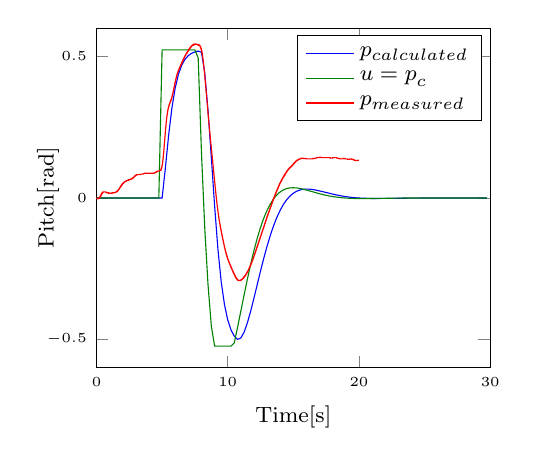
\begin{tikzpicture}

\begin{axis}[%
width = 5cm,
at={(0.758in,0.488in)},
scale only axis,
xmin=0,
xmax=30,
xlabel={\footnotesize{Time[s]}},
ymin=-0.6,
ymax=0.6,
ylabel={\footnotesize{Pitch[rad]}},
ylabel shift = -0.4cm,
axis background/.style={fill=white},
ticklabel style = {font=\tiny},
legend style={legend cell align=left, align=left, draw=black, font = \footnotesize}
]
\addplot [color=blue]
  table[row sep=crcr]{%
0	0\\
5	0\\
5.25	0.106028752058656\\
5.5	0.222660379323177\\
5.75	0.318881471816407\\
6	0.389443606311442\\
6.25	0.437955073776777\\
6.5	0.469972642303901\\
6.75	0.490517248775472\\
7	0.503431001414743\\
7.25	0.511421385860295\\
7.5	0.51630439857702\\
7.75	0.519258621270637\\
8	0.515203257617205\\
8.25	0.442077494057866\\
8.5	0.308917942206627\\
8.75	0.143857437412503\\
9	-0.026642171347433\\
9.25	-0.178852015358114\\
9.5	-0.294706712119982\\
9.75	-0.376103400744807\\
10	-0.430593712461647\\
10.25	-0.465910557041166\\
10.5	-0.488275766784287\\
10.75	-0.499764190883543\\
11	-0.494606006688155\\
11.25	-0.473847629784874\\
11.5	-0.440912018084063\\
11.75	-0.399653357456756\\
12	-0.353578675828111\\
12.5	-0.2579493548984\\
12.75	-0.212334914967485\\
13	-0.169924129646144\\
13.25	-0.131479200507158\\
13.5	-0.0974290818102865\\
13.75	-0.0679368059974763\\
14	-0.0429635308410177\\
14.25	-0.0223192342127767\\
14.5	-0.00570663885556044\\
14.75	0.00724201878417929\\
15	0.0169351049858726\\
15.25	0.0237983108610464\\
15.5	0.0282551996218636\\
15.75	0.03071226238756\\
16	0.0315508532381052\\
16.25	0.0311187961644848\\
16.5	0.029725886927416\\
16.75	0.0276432096833794\\
17.25	0.0222957734120826\\
18.25	0.0110954475341742\\
18.75	0.00659868322602009\\
19.25	0.003167897261946\\
19.75	0.000778241874598962\\
20.25	-0.000708334391688936\\
21	-0.00165871055146738\\
22	-0.00152183353077362\\
25	0\\
29.75	0\\
};
\addlegendentry{$\text{p}_{\text{calculated}}$}

\addplot [color=black!50!green]
  table[row sep=crcr]{%
0	0\\
4.75	0\\
5	0.523598775598298\\
7.5	0.523598775598298\\
7.75	0.494819035995317\\
8	0.160146388213864\\
8.25	-0.106263288038623\\
8.5	-0.307278306480395\\
8.75	-0.451544073993496\\
9	-0.523598775598298\\
10.25	-0.523598775598298\\
10.5	-0.511598967534702\\
10.75	-0.457129956387682\\
11.25	-0.342212060957365\\
11.5	-0.286365657156612\\
11.75	-0.233757373314109\\
12	-0.185424703030396\\
12.25	-0.142014857669654\\
12.5	-0.10385960931001\\
12.75	-0.0710390273514889\\
13	-0.0434270107361172\\
13.25	-0.0207605455327027\\
13.5	-0.0026532057262969\\
13.75	0.0113316469560196\\
14	0.0216778562869422\\
14.25	0.0288792627115377\\
14.5	0.0334210033379279\\
14.75	0.035766054664041\\
15	0.0363476842410009\\
15.25	0.0355551947305592\\
15.5	0.0337310214270481\\
15.75	0.0311830246785298\\
16.25	0.0248856506222559\\
17	0.0150402814094832\\
17.5	0.00942686961320049\\
18	0.00499923826903981\\
18.5	0.0017986264491725\\
19	-0.000289665822503338\\
19.5	-0.0014745362668549\\
20.25	-0.00203640858014609\\
21.25	-0.00156935527676438\\
23.5	-8.39090499056283e-05\\
26.25	0\\
29.75	0\\
};
\addlegendentry{$\text{u = p}_{\text{c}}$}

\addplot [color=red]
  table[row sep=crcr]{%
0	0\\
0.0100000000000016	0\\
0.0120000000000005	-0.00153398078788669\\
0.0579999999999998	-0.00153398078788669\\
0.0599999999999987	-0.00306796157576983\\
0.128	-0.00306796157576983\\
0.129999999999999	-0.00153398078788669\\
0.190000000000001	-0.00153398078788669\\
0.192	0\\
0.225999999999999	0\\
0.228000000000002	0.00153398078788669\\
0.245999999999999	0.00153398078788669\\
0.248000000000001	0.00306796157576983\\
0.266000000000002	0.00306796157576983\\
0.268000000000001	0.00460194236365652\\
0.294	0.00460194236365652\\
0.295999999999999	0.00613592315154321\\
0.308	0.00613592315154321\\
0.309999999999999	0.0076699039394299\\
0.324000000000002	0.0076699039394299\\
0.326000000000001	0.00920388472731304\\
0.34	0.00920388472731304\\
0.341999999999999	0.0107378655151997\\
0.356000000000002	0.0107378655151997\\
0.358000000000001	0.0122718463030864\\
0.361999999999998	0.0122718463030864\\
0.364000000000001	0.0107378655151997\\
0.366	0.0107378655151997\\
0.367999999999999	0.0122718463030864\\
0.382000000000001	0.0122718463030864\\
0.384	0.0138058270909696\\
0.396000000000001	0.0138058270909696\\
0.398	0.0153398078788562\\
0.411999999999999	0.0153398078788562\\
0.414000000000001	0.0168737886667429\\
0.416	0.0168737886667429\\
0.417999999999999	0.0153398078788562\\
0.423999999999999	0.0153398078788562\\
0.425999999999998	0.0168737886667429\\
0.437999999999999	0.0168737886667429\\
0.440000000000001	0.0184077694546261\\
0.446000000000002	0.0184077694546261\\
0.448	0.0168737886667429\\
0.449999999999999	0.0168737886667429\\
0.452000000000002	0.0184077694546261\\
0.466000000000001	0.0184077694546261\\
0.468	0.0199417502425128\\
0.474	0.0199417502425128\\
0.475999999999999	0.0184077694546261\\
0.478000000000002	0.0184077694546261\\
0.48	0.0199417502425128\\
0.481999999999999	0.0199417502425128\\
0.484000000000002	0.0214757310303995\\
0.486000000000001	0.0214757310303995\\
0.488	0.0199417502425128\\
0.494	0.0199417502425128\\
0.495999999999999	0.0214757310303995\\
0.5	0.0214757310303995\\
0.501999999999999	0.0199417502425128\\
0.507999999999999	0.0199417502425128\\
0.510000000000002	0.0214757310303995\\
0.518000000000001	0.0214757310303995\\
0.52	0.0199417502425128\\
0.521999999999998	0.0214757310303995\\
0.710000000000001	0.0214757310303995\\
0.712	0.0199417502425128\\
0.780000000000001	0.0199417502425128\\
0.782	0.0184077694546261\\
0.916	0.0184077694546261\\
0.917999999999999	0.0168737886667429\\
1.19	0.0168737886667429\\
1.192	0.0184077694546261\\
1.396	0.0184077694546261\\
1.398	0.0199417502425128\\
1.472	0.0199417502425128\\
1.474	0.0214757310303995\\
1.524	0.0214757310303995\\
1.526	0.0230097118182861\\
1.58	0.0230097118182861\\
1.582	0.0245436926061693\\
1.608	0.0245436926061693\\
1.61	0.026077673394056\\
1.642	0.026077673394056\\
1.644	0.0276116541819427\\
1.666	0.0276116541819427\\
1.668	0.0291456349698258\\
1.69	0.0291456349698258\\
1.692	0.0306796157577125\\
1.714	0.0306796157577125\\
1.716	0.0322135965455992\\
1.738	0.0322135965455992\\
1.74	0.0337475773334859\\
1.76	0.0337475773334859\\
1.762	0.035281558121369\\
1.782	0.035281558121369\\
1.784	0.0368155389092557\\
1.804	0.0368155389092557\\
1.806	0.0383495196971424\\
1.824	0.0383495196971424\\
1.826	0.0398835004850255\\
1.846	0.0398835004850255\\
1.848	0.0414174812729122\\
1.866	0.0414174812729122\\
1.868	0.0429514620607989\\
1.888	0.0429514620607989\\
1.89	0.0444854428486821\\
1.91	0.0444854428486821\\
1.912	0.0460194236365687\\
1.936	0.0460194236365687\\
1.938	0.0475534044244554\\
1.962	0.0475534044244554\\
1.964	0.0490873852123421\\
1.986	0.0490873852123421\\
1.988	0.0506213660002253\\
2.012	0.0506213660002253\\
2.014	0.052155346788112\\
2.048	0.052155346788112\\
2.05	0.0536893275759986\\
2.082	0.0536893275759986\\
2.084	0.0552233083638818\\
2.128	0.0552233083638818\\
2.13	0.0567572891517685\\
2.166	0.0567572891517685\\
2.168	0.0582912699396552\\
2.224	0.0582912699396552\\
2.226	0.0598252507275383\\
2.276	0.0598252507275383\\
2.278	0.061359231515425\\
2.354	0.061359231515425\\
2.356	0.0628932123033117\\
2.446	0.0628932123033117\\
2.448	0.0644271930911984\\
2.548	0.0644271930911984\\
2.55	0.0659611738790815\\
2.628	0.0659611738790815\\
2.63	0.0674951546669682\\
2.698	0.0674951546669682\\
2.7	0.0690291354548549\\
2.746	0.0690291354548549\\
2.748	0.070563116242738\\
2.79	0.070563116242738\\
2.792	0.0720970970306247\\
2.832	0.0720970970306247\\
2.834	0.0736310778185114\\
2.864	0.0736310778185114\\
2.866	0.0751650586063981\\
2.896	0.0751650586063981\\
2.898	0.0766990393942812\\
2.93	0.0766990393942812\\
2.932	0.0782330201821679\\
2.97	0.0782330201821679\\
2.972	0.0797670009700546\\
3.012	0.0797670009700546\\
3.014	0.0813009817579378\\
3.056	0.0813009817579378\\
3.058	0.0828349625458245\\
3.356	0.0828349625458245\\
3.358	0.0843689433337111\\
3.554	0.0843689433337111\\
3.556	0.0859029241215943\\
3.668	0.0859029241215943\\
3.67	0.087436904909481\\
4.386	0.087436904909481\\
4.388	0.0889708856973677\\
4.472	0.0889708856973677\\
4.474	0.0905048664852544\\
4.53	0.0905048664852544\\
4.532	0.0920388472731375\\
4.588	0.0920388472731375\\
4.59	0.0935728280610242\\
4.652	0.0935728280610242\\
4.654	0.0951068088489109\\
4.77	0.0951068088489109\\
4.772	0.096640789636794\\
4.874	0.096640789636794\\
4.876	0.0981747704246807\\
4.902	0.0981747704246807\\
4.904	0.0997087512125674\\
4.916	0.0997087512125674\\
4.918	0.101242732000454\\
4.93	0.101242732000454\\
4.932	0.102776712788337\\
4.944	0.102776712788337\\
4.946	0.104310693576224\\
4.954	0.104310693576224\\
4.956	0.105844674364111\\
4.964	0.105844674364111\\
4.966	0.107378655151994\\
4.974	0.107378655151994\\
4.976	0.10891263593988\\
4.978	0.10891263593988\\
4.98	0.110446616727767\\
4.988	0.110446616727767\\
4.992	0.113514578303537\\
5	0.113514578303537\\
5.002	0.115048559091424\\
5.004	0.115048559091424\\
5.006	0.11658253987931\\
5.012	0.11658253987931\\
5.016	0.11965050145508\\
5.022	0.11965050145508\\
5.024	0.121184482242967\\
5.026	0.121184482242967\\
5.028	0.12271846303085\\
5.03	0.12271846303085\\
5.032	0.124252443818737\\
5.036	0.124252443818737\\
5.038	0.125786424606623\\
5.04	0.125786424606623\\
5.042	0.127320405394507\\
5.044	0.127320405394507\\
5.046	0.128854386182393\\
5.048	0.128854386182393\\
5.05	0.13038836697028\\
5.052	0.13038836697028\\
5.054	0.131922347758167\\
5.056	0.131922347758167\\
5.058	0.13345632854605\\
5.06	0.13345632854605\\
5.062	0.134990309333936\\
5.064	0.134990309333936\\
5.066	0.136524290121823\\
5.068	0.136524290121823\\
5.07	0.138058270909706\\
5.072	0.138058270909706\\
5.076	0.14112623248548\\
5.078	0.14112623248548\\
5.08	0.142660213273366\\
5.082	0.142660213273366\\
5.084	0.144194194061249\\
5.086	0.144194194061249\\
5.09	0.147262155637023\\
5.092	0.147262155637023\\
5.094	0.148796136424906\\
5.096	0.148796136424906\\
5.1	0.151864098000679\\
5.102	0.151864098000679\\
5.106	0.154932059576449\\
5.108	0.154932059576449\\
5.112	0.158000021152223\\
5.114	0.158000021152223\\
5.116	0.159534001940106\\
5.118	0.159534001940106\\
5.122	0.162601963515879\\
5.124	0.162601963515879\\
5.13	0.167203905879536\\
5.132	0.167203905879536\\
5.138	0.171805848243192\\
5.14	0.171805848243192\\
5.142	0.173339829031079\\
5.144	0.173339829031079\\
5.152	0.179475752182618\\
5.154	0.179475752182618\\
5.156	0.181009732970505\\
5.158	0.181009732970505\\
5.166	0.187145656122048\\
5.168	0.187145656122048\\
5.17	0.188679636909935\\
5.172	0.188679636909935\\
5.18	0.194815560061475\\
5.182	0.194815560061475\\
5.19	0.200951483213018\\
5.194	0.200951483213018\\
5.204	0.208621387152448\\
5.206	0.208621387152448\\
5.212	0.213223329516104\\
5.214	0.213223329516104\\
5.218	0.216291291091874\\
5.22	0.216291291091874\\
5.228	0.222427214243417\\
5.23	0.222427214243417\\
5.232	0.223961195031304\\
5.234	0.223961195031304\\
5.242	0.230097118182847\\
5.244	0.230097118182847\\
5.248	0.233165079758617\\
5.25	0.233165079758617\\
5.254	0.23623304133439\\
5.256	0.23623304133439\\
5.264	0.24236896448593\\
5.266	0.24236896448593\\
5.268	0.243902945273817\\
5.27	0.243902945273817\\
5.278	0.25003886842536\\
5.282	0.25003886842536\\
5.29	0.256174791576903\\
5.296	0.256174791576903\\
5.298	0.257708772364786\\
5.3	0.26077673394056\\
5.302	0.262310714728443\\
5.308	0.262310714728443\\
5.316	0.268446637879986\\
5.32	0.268446637879986\\
5.326	0.273048580243643\\
5.332	0.273048580243643\\
5.34	0.279184503395186\\
5.346	0.279184503395186\\
5.352	0.283786445758842\\
5.358	0.283786445758842\\
5.364	0.288388388122499\\
5.37	0.288388388122499\\
5.376	0.292990330486159\\
5.378	0.292990330486159\\
5.38	0.291456349698272\\
5.388	0.297592272849815\\
5.39	0.296058292061929\\
5.394	0.296058292061929\\
5.4	0.300660234425585\\
5.402	0.300660234425585\\
5.404	0.299126253637699\\
5.406	0.299126253637699\\
5.408	0.300660234425585\\
5.41	0.303728196001359\\
5.412	0.303728196001359\\
5.414	0.305262176789242\\
5.416	0.303728196001359\\
5.418	0.303728196001359\\
5.424	0.308330138365015\\
5.426	0.308330138365015\\
5.428	0.306796157577129\\
5.43	0.306796157577129\\
5.436	0.311398099940785\\
5.438	0.311398099940785\\
5.44	0.309864119152898\\
5.442	0.309864119152898\\
5.446	0.312932080728672\\
5.448	0.312932080728672\\
5.45	0.314466061516555\\
5.452	0.312932080728672\\
5.456	0.312932080728672\\
5.46	0.316000042304442\\
5.468	0.316000042304442\\
5.472	0.319068003880215\\
5.476	0.319068003880215\\
5.478	0.317534023092328\\
5.48	0.317534023092328\\
5.486	0.322135965455985\\
5.488	0.320601984668098\\
5.494	0.320601984668098\\
5.498	0.323669946243871\\
5.5	0.323669946243871\\
5.502	0.322135965455985\\
5.504	0.322135965455985\\
5.506	0.323669946243871\\
5.508	0.323669946243871\\
5.51	0.325203927031755\\
5.514	0.325203927031755\\
5.516	0.323669946243871\\
5.518	0.325203927031755\\
5.52	0.325203927031755\\
5.522	0.326737907819641\\
5.53	0.326737907819641\\
5.532	0.328271888607528\\
5.542	0.328271888607528\\
5.544	0.329805869395411\\
5.554	0.329805869395411\\
5.556	0.331339850183298\\
5.566	0.331339850183298\\
5.568	0.332873830971185\\
5.578	0.332873830971185\\
5.58	0.334407811759071\\
5.59	0.334407811759071\\
5.592	0.335941792546954\\
5.602	0.335941792546954\\
5.604	0.337475773334841\\
5.616	0.337475773334841\\
5.618	0.339009754122728\\
5.628	0.339009754122728\\
5.63	0.340543734910611\\
5.642	0.340543734910611\\
5.644	0.342077715698498\\
5.654	0.342077715698498\\
5.656	0.343611696486384\\
5.666	0.343611696486384\\
5.668	0.345145677274271\\
5.676	0.345145677274271\\
5.678	0.346679658062154\\
5.688	0.346679658062154\\
5.69	0.348213638850041\\
5.7	0.348213638850041\\
5.702	0.349747619637927\\
5.712	0.349747619637927\\
5.714	0.351281600425811\\
5.722	0.351281600425811\\
5.724	0.352815581213697\\
5.73	0.352815581213697\\
5.732	0.354349562001584\\
5.738	0.354349562001584\\
5.74	0.355883542789467\\
5.748	0.355883542789467\\
5.75	0.357417523577354\\
5.758	0.357417523577354\\
5.76	0.35895150436524\\
5.766	0.35895150436524\\
5.768	0.360485485153127\\
5.774	0.360485485153127\\
5.776	0.36201946594101\\
5.784	0.36201946594101\\
5.786	0.363553446728897\\
5.79	0.363553446728897\\
5.792	0.365087427516784\\
5.798	0.365087427516784\\
5.8	0.366621408304667\\
5.806	0.366621408304667\\
5.808	0.368155389092554\\
5.816	0.368155389092554\\
5.818	0.36968936988044\\
5.82	0.36968936988044\\
5.822	0.371223350668327\\
5.83	0.371223350668327\\
5.832	0.37275733145621\\
5.834	0.37275733145621\\
5.836	0.374291312244097\\
5.844	0.374291312244097\\
5.846	0.375825293031983\\
5.85	0.375825293031983\\
5.852	0.377359273819867\\
5.858	0.377359273819867\\
5.86	0.378893254607753\\
5.864	0.378893254607753\\
5.866	0.38042723539564\\
5.872	0.38042723539564\\
5.874	0.381961216183523\\
5.878	0.381961216183523\\
5.88	0.38349519697141\\
5.886	0.38349519697141\\
5.888	0.385029177759296\\
5.892	0.385029177759296\\
5.894	0.386563158547183\\
5.9	0.386563158547183\\
5.902	0.388097139335066\\
5.906	0.388097139335066\\
5.908	0.389631120122953\\
5.914	0.389631120122953\\
5.916	0.39116510091084\\
5.918	0.39116510091084\\
5.92	0.392699081698723\\
5.928	0.392699081698723\\
5.93	0.394233062486609\\
5.932	0.394233062486609\\
5.934	0.395767043274496\\
5.94	0.395767043274496\\
5.942	0.397301024062379\\
5.948	0.397301024062379\\
5.95	0.398835004850266\\
5.954	0.398835004850266\\
5.956	0.400368985638153\\
5.96	0.400368985638153\\
5.962	0.401902966426039\\
5.968	0.401902966426039\\
5.97	0.403436947213923\\
5.974	0.403436947213923\\
5.976	0.404970928001809\\
5.982	0.404970928001809\\
5.984	0.406504908789696\\
5.988	0.406504908789696\\
5.99	0.408038889577579\\
5.996	0.408038889577579\\
5.998	0.409572870365466\\
6.002	0.409572870365466\\
6.004	0.411106851153352\\
6.01	0.411106851153352\\
6.012	0.412640831941239\\
6.016	0.412640831941239\\
6.018	0.414174812729122\\
6.024	0.414174812729122\\
6.026	0.415708793517009\\
6.032	0.415708793517009\\
6.034	0.417242774304896\\
6.04	0.417242774304896\\
6.042	0.418776755092779\\
6.046	0.418776755092779\\
6.048	0.420310735880665\\
6.054	0.420310735880665\\
6.056	0.421844716668552\\
6.062	0.421844716668552\\
6.064	0.423378697456435\\
6.07	0.423378697456435\\
6.072	0.424912678244322\\
6.078	0.424912678244322\\
6.08	0.426446659032209\\
6.086	0.426446659032209\\
6.088	0.427980639820095\\
6.096	0.427980639820095\\
6.098	0.429514620607979\\
6.104	0.429514620607979\\
6.106	0.431048601395865\\
6.114	0.431048601395865\\
6.116	0.432582582183752\\
6.122	0.432582582183752\\
6.124	0.434116562971635\\
6.132	0.434116562971635\\
6.134	0.435650543759522\\
6.142	0.435650543759522\\
6.144	0.437184524547408\\
6.152	0.437184524547408\\
6.154	0.438718505335295\\
6.162	0.438718505335295\\
6.164	0.440252486123178\\
6.172	0.440252486123178\\
6.174	0.441786466911065\\
6.184	0.441786466911065\\
6.186	0.443320447698952\\
6.194	0.443320447698952\\
6.196	0.444854428486835\\
6.206	0.444854428486835\\
6.208	0.446388409274721\\
6.218	0.446388409274721\\
6.22	0.447922390062608\\
6.23	0.447922390062608\\
6.232	0.449456370850491\\
6.244	0.449456370850491\\
6.246	0.450990351638378\\
6.258	0.450990351638378\\
6.26	0.452524332426265\\
6.27	0.452524332426265\\
6.272	0.454058313214151\\
6.284	0.454058313214151\\
6.286	0.455592294002034\\
6.298	0.455592294002034\\
6.3	0.457126274789921\\
6.312	0.457126274789921\\
6.314	0.458660255577808\\
6.324	0.458660255577808\\
6.326	0.460194236365691\\
6.34	0.460194236365691\\
6.342	0.461728217153578\\
6.354	0.461728217153578\\
6.356	0.463262197941464\\
6.374	0.463262197941464\\
6.376	0.464796178729351\\
6.386	0.464796178729351\\
6.388	0.466330159517234\\
6.4	0.466330159517234\\
6.402	0.467864140305121\\
6.414	0.467864140305121\\
6.416	0.469398121093008\\
6.428	0.469398121093008\\
6.43	0.470932101880891\\
6.442	0.470932101880891\\
6.444	0.472466082668777\\
6.464	0.472466082668777\\
6.466	0.474000063456664\\
6.476	0.474000063456664\\
6.478	0.475534044244547\\
6.49	0.475534044244547\\
6.492	0.477068025032434\\
6.502	0.477068025032434\\
6.504	0.478602005820321\\
6.516	0.478602005820321\\
6.518	0.480135986608207\\
6.53	0.480135986608207\\
6.532	0.48166996739609\\
6.536	0.48166996739609\\
6.538	0.480135986608207\\
6.54	0.48166996739609\\
6.552	0.48166996739609\\
6.554	0.483203948183977\\
6.566	0.483203948183977\\
6.568	0.484737928971864\\
6.578	0.484737928971864\\
6.58	0.486271909759747\\
6.592	0.486271909759747\\
6.594	0.487805890547634\\
6.614	0.487805890547634\\
6.616	0.48933987133552\\
6.626	0.48933987133552\\
6.628	0.490873852123404\\
6.64	0.490873852123404\\
6.642	0.49240783291129\\
6.654	0.49240783291129\\
6.656	0.493941813699177\\
6.672	0.493941813699177\\
6.674	0.495475794487064\\
6.688	0.495475794487064\\
6.69	0.497009775274947\\
6.704	0.497009775274947\\
6.706	0.498543756062833\\
6.722	0.498543756062833\\
6.724	0.50007773685072\\
6.738	0.50007773685072\\
6.74	0.501611717638603\\
6.76	0.501611717638603\\
6.762	0.50314569842649\\
6.774	0.50314569842649\\
6.776	0.504679679214377\\
6.79	0.504679679214377\\
6.792	0.506213660002263\\
6.794	0.506213660002263\\
6.796	0.504679679214377\\
6.798	0.504679679214377\\
6.8	0.506213660002263\\
6.812	0.506213660002263\\
6.814	0.507747640790146\\
6.826	0.507747640790146\\
6.828	0.509281621578033\\
6.83	0.509281621578033\\
6.832	0.507747640790146\\
6.836	0.507747640790146\\
6.838	0.509281621578033\\
6.85	0.509281621578033\\
6.852	0.51081560236592\\
6.858	0.51081560236592\\
6.86	0.509281621578033\\
6.862	0.51081560236592\\
6.864	0.51081560236592\\
6.866	0.512349583153803\\
6.868	0.512349583153803\\
6.87	0.51081560236592\\
6.874	0.51081560236592\\
6.876	0.512349583153803\\
6.888	0.512349583153803\\
6.89	0.51388356394169\\
6.894	0.51388356394169\\
6.896	0.512349583153803\\
6.898	0.512349583153803\\
6.9	0.51388356394169\\
6.912	0.51388356394169\\
6.914	0.515417544729576\\
6.926	0.515417544729576\\
6.928	0.516951525517459\\
6.93	0.516951525517459\\
6.932	0.515417544729576\\
6.936	0.515417544729576\\
6.938	0.516951525517459\\
6.95	0.516951525517459\\
6.952	0.518485506305346\\
6.958	0.518485506305346\\
6.96	0.516951525517459\\
6.962	0.518485506305346\\
6.966	0.518485506305346\\
6.968	0.520019487093233\\
6.97	0.518485506305346\\
6.974	0.518485506305346\\
6.976	0.520019487093233\\
6.988	0.520019487093233\\
6.99	0.52155346788112\\
6.994	0.52155346788112\\
6.996	0.520019487093233\\
6.998	0.520019487093233\\
7	0.52155346788112\\
7.012	0.52155346788112\\
7.014	0.523087448669003\\
7.026	0.523087448669003\\
7.028	0.524621429456889\\
7.03	0.524621429456889\\
7.032	0.523087448669003\\
7.036	0.523087448669003\\
7.038	0.524621429456889\\
7.052	0.524621429456889\\
7.054	0.526155410244776\\
7.056	0.526155410244776\\
7.058	0.524621429456889\\
7.06	0.524621429456889\\
7.062	0.526155410244776\\
7.074	0.526155410244776\\
7.076	0.527689391032659\\
7.1	0.527689391032659\\
7.102	0.529223371820546\\
7.116	0.529223371820546\\
7.118	0.530757352608433\\
7.12	0.529223371820546\\
7.124	0.529223371820546\\
7.126	0.530757352608433\\
7.148	0.530757352608433\\
7.15	0.532291333396319\\
7.174	0.532291333396319\\
7.176	0.533825314184202\\
7.2	0.533825314184202\\
7.202	0.535359294972089\\
7.23	0.535359294972089\\
7.232	0.536893275759976\\
7.268	0.536893275759976\\
7.27	0.538427256547859\\
7.294	0.538427256547859\\
7.296	0.539961237335746\\
7.298	0.539961237335746\\
7.3	0.538427256547859\\
7.304	0.538427256547859\\
7.306	0.539961237335746\\
7.332	0.539961237335746\\
7.334	0.541495218123632\\
7.336	0.539961237335746\\
7.342	0.539961237335746\\
7.344	0.541495218123632\\
7.348	0.541495218123632\\
7.35	0.539961237335746\\
7.354	0.539961237335746\\
7.356	0.541495218123632\\
7.362	0.541495218123632\\
7.364	0.539961237335746\\
7.366	0.541495218123632\\
7.38	0.541495218123632\\
7.382	0.543029198911515\\
7.384	0.543029198911515\\
7.386	0.541495218123632\\
7.392	0.541495218123632\\
7.394	0.543029198911515\\
7.398	0.543029198911515\\
7.4	0.541495218123632\\
7.404	0.541495218123632\\
7.406	0.543029198911515\\
7.41	0.543029198911515\\
7.412	0.541495218123632\\
7.416	0.541495218123632\\
7.418	0.543029198911515\\
7.422	0.543029198911515\\
7.424	0.541495218123632\\
7.428	0.541495218123632\\
7.43	0.543029198911515\\
7.436	0.543029198911515\\
7.438	0.541495218123632\\
7.44	0.541495218123632\\
7.444	0.544563179699402\\
7.446	0.544563179699402\\
7.45	0.541495218123632\\
7.452	0.541495218123632\\
7.456	0.544563179699402\\
7.458	0.544563179699402\\
7.462	0.541495218123632\\
7.464	0.541495218123632\\
7.468	0.544563179699402\\
7.47	0.544563179699402\\
7.474	0.541495218123632\\
7.476	0.541495218123632\\
7.48	0.544563179699402\\
7.482	0.544563179699402\\
7.484	0.543029198911515\\
7.486	0.543029198911515\\
7.488	0.541495218123632\\
7.492	0.544563179699402\\
7.496	0.544563179699402\\
7.498	0.543029198911515\\
7.502	0.543029198911515\\
7.504	0.544563179699402\\
7.508	0.544563179699402\\
7.51	0.543029198911515\\
7.514	0.543029198911515\\
7.516	0.544563179699402\\
7.52	0.544563179699402\\
7.522	0.543029198911515\\
7.526	0.543029198911515\\
7.528	0.544563179699402\\
7.532	0.544563179699402\\
7.534	0.543029198911515\\
7.538	0.543029198911515\\
7.54	0.544563179699402\\
7.544	0.544563179699402\\
7.546	0.543029198911515\\
7.552	0.543029198911515\\
7.554	0.544563179699402\\
7.556	0.544563179699402\\
7.558	0.543029198911515\\
7.564	0.543029198911515\\
7.566	0.544563179699402\\
7.568	0.544563179699402\\
7.57	0.543029198911515\\
7.576	0.543029198911515\\
7.578	0.544563179699402\\
7.58	0.544563179699402\\
7.582	0.543029198911515\\
7.588	0.543029198911515\\
7.59	0.544563179699402\\
7.592	0.543029198911515\\
7.646	0.543029198911515\\
7.648	0.544563179699402\\
7.65	0.543029198911515\\
7.658	0.543029198911515\\
7.66	0.544563179699402\\
7.662	0.543029198911515\\
7.67	0.543029198911515\\
7.672	0.544563179699402\\
7.674	0.543029198911515\\
7.676	0.543029198911515\\
7.678	0.541495218123632\\
7.68	0.543029198911515\\
7.682	0.543029198911515\\
7.684	0.544563179699402\\
7.688	0.541495218123632\\
7.69	0.541495218123632\\
7.692	0.543029198911515\\
7.694	0.543029198911515\\
7.696	0.544563179699402\\
7.7	0.541495218123632\\
7.702	0.541495218123632\\
7.704	0.543029198911515\\
7.706	0.543029198911515\\
7.708	0.544563179699402\\
7.712	0.541495218123632\\
7.716	0.541495218123632\\
7.718	0.543029198911515\\
7.722	0.543029198911515\\
7.724	0.541495218123632\\
7.728	0.541495218123632\\
7.73	0.543029198911515\\
7.734	0.543029198911515\\
7.736	0.541495218123632\\
7.74	0.541495218123632\\
7.742	0.543029198911515\\
7.746	0.543029198911515\\
7.748	0.541495218123632\\
7.754	0.541495218123632\\
7.756	0.543029198911515\\
7.758	0.543029198911515\\
7.762	0.539961237335746\\
7.764	0.541495218123632\\
7.766	0.541495218123632\\
7.768	0.543029198911515\\
7.77	0.543029198911515\\
7.774	0.539961237335746\\
7.776	0.539961237335746\\
7.778	0.541495218123632\\
7.784	0.541495218123632\\
7.786	0.539961237335746\\
7.788	0.539961237335746\\
7.79	0.541495218123632\\
7.796	0.541495218123632\\
7.798	0.539961237335746\\
7.802	0.539961237335746\\
7.804	0.541495218123632\\
7.806	0.541495218123632\\
7.808	0.539961237335746\\
7.84	0.539961237335746\\
7.842	0.538427256547859\\
7.844	0.538427256547859\\
7.846	0.539961237335746\\
7.848	0.539961237335746\\
7.85	0.538427256547859\\
7.864	0.538427256547859\\
7.866	0.536893275759976\\
7.868	0.538427256547859\\
7.874	0.538427256547859\\
7.876	0.536893275759976\\
7.882	0.536893275759976\\
7.884	0.538427256547859\\
7.886	0.536893275759976\\
7.888	0.536893275759976\\
7.89	0.535359294972089\\
7.892	0.536893275759976\\
7.898	0.536893275759976\\
7.9	0.535359294972089\\
7.906	0.535359294972089\\
7.908	0.536893275759976\\
7.912	0.533825314184202\\
7.916	0.533825314184202\\
7.918	0.535359294972089\\
7.922	0.535359294972089\\
7.926	0.532291333396319\\
7.928	0.532291333396319\\
7.93	0.533825314184202\\
7.934	0.533825314184202\\
7.938	0.530757352608433\\
7.94	0.530757352608433\\
7.944	0.533825314184202\\
7.95	0.529223371820546\\
7.952	0.529223371820546\\
7.956	0.532291333396319\\
7.962	0.527689391032659\\
7.964	0.527689391032659\\
7.968	0.530757352608433\\
7.974	0.526155410244776\\
7.976	0.526155410244776\\
7.978	0.527689391032659\\
7.982	0.527689391032659\\
7.986	0.524621429456889\\
7.99	0.524621429456889\\
7.992	0.526155410244776\\
7.994	0.526155410244776\\
7.996	0.524621429456889\\
7.998	0.52155346788112\\
8	0.52155346788112\\
8.004	0.524621429456889\\
8.01	0.520019487093233\\
8.014	0.520019487093233\\
8.016	0.52155346788112\\
8.018	0.52155346788112\\
8.02	0.520019487093233\\
8.022	0.516951525517459\\
8.026	0.516951525517459\\
8.028	0.518485506305346\\
8.03	0.518485506305346\\
8.032	0.516951525517459\\
8.034	0.51388356394169\\
8.036	0.51388356394169\\
8.038	0.515417544729576\\
8.042	0.515417544729576\\
8.048	0.51081560236592\\
8.05	0.512349583153803\\
8.054	0.512349583153803\\
8.06	0.507747640790146\\
8.062	0.507747640790146\\
8.064	0.509281621578033\\
8.066	0.509281621578033\\
8.068	0.507747640790146\\
8.07	0.504679679214377\\
8.074	0.504679679214377\\
8.076	0.506213660002263\\
8.082	0.501611717638603\\
8.09	0.501611717638603\\
8.096	0.497009775274947\\
8.102	0.497009775274947\\
8.106	0.493941813699177\\
8.112	0.493941813699177\\
8.118	0.48933987133552\\
8.124	0.48933987133552\\
8.128	0.486271909759747\\
8.13	0.486271909759747\\
8.132	0.484737928971864\\
8.136	0.484737928971864\\
8.14	0.48166996739609\\
8.146	0.48166996739609\\
8.154	0.475534044244547\\
8.16	0.475534044244547\\
8.166	0.470932101880891\\
8.17	0.470932101880891\\
8.176	0.466330159517234\\
8.182	0.466330159517234\\
8.188	0.461728217153578\\
8.194	0.461728217153578\\
8.196	0.460194236365691\\
8.198	0.457126274789921\\
8.2	0.455592294002034\\
8.206	0.455592294002034\\
8.214	0.449456370850491\\
8.216	0.449456370850491\\
8.218	0.450990351638378\\
8.22	0.449456370850491\\
8.222	0.446388409274721\\
8.224	0.444854428486835\\
8.23	0.444854428486835\\
8.232	0.443320447698952\\
8.234	0.440252486123178\\
8.236	0.438718505335295\\
8.242	0.438718505335295\\
8.244	0.437184524547408\\
8.246	0.434116562971635\\
8.248	0.432582582183752\\
8.254	0.432582582183752\\
8.258	0.429514620607979\\
8.26	0.426446659032209\\
8.266	0.426446659032209\\
8.27	0.423378697456435\\
8.272	0.420310735880665\\
8.28	0.420310735880665\\
8.284	0.414174812729122\\
8.292	0.414174812729122\\
8.294	0.411106851153352\\
8.298	0.408038889577579\\
8.304	0.408038889577579\\
8.308	0.401902966426039\\
8.316	0.401902966426039\\
8.32	0.395767043274496\\
8.326	0.395767043274496\\
8.33	0.392699081698723\\
8.332	0.389631120122953\\
8.338	0.389631120122953\\
8.342	0.386563158547183\\
8.344	0.38349519697141\\
8.346	0.381961216183523\\
8.352	0.381961216183523\\
8.354	0.38042723539564\\
8.356	0.377359273819867\\
8.358	0.375825293031983\\
8.364	0.375825293031983\\
8.366	0.374291312244097\\
8.368	0.371223350668327\\
8.37	0.36968936988044\\
8.374	0.36968936988044\\
8.382	0.363553446728897\\
8.384	0.363553446728897\\
8.386	0.36201946594101\\
8.388	0.36201946594101\\
8.396	0.355883542789467\\
8.398	0.355883542789467\\
8.4	0.354349562001584\\
8.402	0.354349562001584\\
8.408	0.349747619637927\\
8.41	0.349747619637927\\
8.414	0.346679658062154\\
8.416	0.346679658062154\\
8.422	0.342077715698498\\
8.424	0.342077715698498\\
8.428	0.339009754122728\\
8.43	0.339009754122728\\
8.436	0.334407811759071\\
8.438	0.334407811759071\\
8.442	0.331339850183298\\
8.444	0.331339850183298\\
8.45	0.326737907819641\\
8.452	0.326737907819641\\
8.454	0.325203927031755\\
8.456	0.325203927031755\\
8.464	0.319068003880215\\
8.466	0.319068003880215\\
8.472	0.314466061516555\\
8.474	0.314466061516555\\
8.476	0.312932080728672\\
8.478	0.312932080728672\\
8.486	0.306796157577129\\
8.49	0.306796157577129\\
8.498	0.300660234425585\\
8.5	0.300660234425585\\
8.502	0.299126253637699\\
8.504	0.299126253637699\\
8.51	0.294524311274042\\
8.512	0.294524311274042\\
8.514	0.292990330486159\\
8.516	0.292990330486159\\
8.524	0.286854407334616\\
8.526	0.286854407334616\\
8.528	0.285320426546729\\
8.53	0.285320426546729\\
8.536	0.280718484183073\\
8.538	0.280718484183073\\
8.54	0.279184503395186\\
8.542	0.279184503395186\\
8.548	0.274582561031529\\
8.55	0.274582561031529\\
8.554	0.27151459945576\\
8.556	0.27151459945576\\
8.56	0.268446637879986\\
8.562	0.268446637879986\\
8.568	0.26384469551633\\
8.572	0.26384469551633\\
8.58	0.257708772364786\\
8.584	0.257708772364786\\
8.586	0.256174791576903\\
8.588	0.256174791576903\\
8.59	0.254640810789017\\
8.592	0.251572849213247\\
8.596	0.251572849213247\\
8.598	0.25003886842536\\
8.6	0.25003886842536\\
8.602	0.248504887637473\\
8.604	0.245436926061704\\
8.608	0.245436926061704\\
8.61	0.243902945273817\\
8.612	0.243902945273817\\
8.618	0.23930100291016\\
8.62	0.23930100291016\\
8.622	0.237767022122274\\
8.624	0.237767022122274\\
8.63	0.233165079758617\\
8.634	0.233165079758617\\
8.642	0.227029156607074\\
8.646	0.227029156607074\\
8.648	0.225495175819191\\
8.65	0.225495175819191\\
8.656	0.220893233455531\\
8.66	0.220893233455531\\
8.668	0.214757310303991\\
8.672	0.214757310303991\\
8.678	0.210155367940335\\
8.68	0.210155367940335\\
8.682	0.208621387152448\\
8.684	0.208621387152448\\
8.688	0.205553425576674\\
8.69	0.205553425576674\\
8.692	0.204019444788791\\
8.694	0.204019444788791\\
8.696	0.202485464000905\\
8.698	0.202485464000905\\
8.704	0.197883521637248\\
8.708	0.197883521637248\\
8.714	0.193281579273592\\
8.716	0.193281579273592\\
8.718	0.191747598485705\\
8.72	0.191747598485705\\
8.726	0.187145656122048\\
8.732	0.187145656122048\\
8.74	0.181009732970505\\
8.744	0.181009732970505\\
8.75	0.176407790606849\\
8.754	0.176407790606849\\
8.756	0.174873809818962\\
8.758	0.174873809818962\\
8.76	0.173339829031079\\
8.762	0.170271867455305\\
8.768	0.170271867455305\\
8.776	0.164135944303762\\
8.782	0.164135944303762\\
8.784	0.161067982727992\\
8.786	0.159534001940106\\
8.792	0.159534001940106\\
8.8	0.153398078788562\\
8.806	0.153398078788562\\
8.808	0.150330117212793\\
8.812	0.147262155637023\\
8.818	0.147262155637023\\
8.826	0.14112623248548\\
8.832	0.14112623248548\\
8.834	0.138058270909706\\
8.836	0.136524290121823\\
8.842	0.136524290121823\\
8.846	0.13345632854605\\
8.848	0.13038836697028\\
8.856	0.13038836697028\\
8.858	0.127320405394507\\
8.862	0.124252443818737\\
8.868	0.124252443818737\\
8.87	0.12271846303085\\
8.872	0.11965050145508\\
8.874	0.118116520667193\\
8.88	0.118116520667193\\
8.886	0.113514578303537\\
8.892	0.113514578303537\\
8.894	0.11198059751565\\
8.896	0.10891263593988\\
8.898	0.107378655151994\\
8.904	0.107378655151994\\
8.912	0.101242732000454\\
8.918	0.101242732000454\\
8.92	0.0981747704246807\\
8.924	0.0951068088489109\\
8.93	0.0951068088489109\\
8.932	0.0935728280610242\\
8.934	0.0905048664852544\\
8.936	0.0889708856973677\\
8.942	0.0889708856973677\\
8.948	0.0843689433337111\\
8.954	0.0843689433337111\\
8.956	0.0828349625458245\\
8.958	0.0797670009700546\\
8.96	0.0782330201821679\\
8.966	0.0782330201821679\\
8.974	0.0720970970306247\\
8.98	0.0720970970306247\\
8.982	0.0690291354548549\\
8.986	0.0659611738790815\\
8.992	0.0659611738790815\\
8.994	0.0644271930911984\\
8.996	0.061359231515425\\
8.998	0.061359231515425\\
9	0.0598252507275383\\
9.004	0.0598252507275383\\
9.01	0.0552233083638818\\
9.014	0.0552233083638818\\
9.016	0.0536893275759986\\
9.018	0.0536893275759986\\
9.02	0.0506213660002253\\
9.022	0.0490873852123421\\
9.028	0.0490873852123421\\
9.036	0.0429514620607989\\
9.04	0.0429514620607989\\
9.046	0.0383495196971424\\
9.05	0.0383495196971424\\
9.052	0.0368155389092557\\
9.054	0.0368155389092557\\
9.06	0.0322135965455992\\
9.064	0.0322135965455992\\
9.07	0.0276116541819427\\
9.072	0.0276116541819427\\
9.074	0.026077673394056\\
9.078	0.026077673394056\\
9.084	0.0214757310303995\\
9.088	0.0214757310303995\\
9.094	0.0168737886667429\\
9.096	0.0168737886667429\\
9.098	0.0153398078788562\\
9.102	0.0153398078788562\\
9.108	0.0107378655151997\\
9.112	0.0107378655151997\\
9.116	0.0076699039394299\\
9.118	0.0076699039394299\\
9.12	0.00613592315154321\\
9.122	0.00613592315154321\\
9.124	0.00460194236365652\\
9.126	0.00460194236365652\\
9.13	0.00153398078788669\\
9.132	0.00153398078788669\\
9.134	0\\
9.136	0\\
9.138	-0.00153398078788669\\
9.14	-0.00153398078788669\\
9.144	-0.00460194236365652\\
9.148	-0.00460194236365652\\
9.154	-0.00920388472731304\\
9.16	-0.00920388472731304\\
9.166	-0.0138058270909696\\
9.168	-0.0138058270909696\\
9.17	-0.0153398078788562\\
9.174	-0.0153398078788562\\
9.18	-0.0199417502425128\\
9.186	-0.0199417502425128\\
9.192	-0.0245436926061693\\
9.198	-0.0245436926061693\\
9.204	-0.0291456349698258\\
9.21	-0.0291456349698258\\
9.216	-0.0337475773334859\\
9.222	-0.0337475773334859\\
9.228	-0.0383495196971424\\
9.236	-0.0383495196971424\\
9.242	-0.0429514620607989\\
9.248	-0.0429514620607989\\
9.254	-0.0475534044244554\\
9.26	-0.0475534044244554\\
9.264	-0.0506213660002253\\
9.266	-0.0506213660002253\\
9.268	-0.052155346788112\\
9.274	-0.052155346788112\\
9.278	-0.0552233083638818\\
9.284	-0.0552233083638818\\
9.288	-0.0582912699396552\\
9.29	-0.0582912699396552\\
9.292	-0.0598252507275383\\
9.296	-0.0598252507275383\\
9.298	-0.061359231515425\\
9.3	-0.061359231515425\\
9.302	-0.0628932123033117\\
9.306	-0.0628932123033117\\
9.308	-0.0644271930911984\\
9.31	-0.0644271930911984\\
9.312	-0.0659611738790815\\
9.314	-0.0659611738790815\\
9.316	-0.0674951546669682\\
9.322	-0.0674951546669682\\
9.326	-0.070563116242738\\
9.332	-0.070563116242738\\
9.336	-0.0736310778185114\\
9.338	-0.0736310778185114\\
9.34	-0.0751650586063981\\
9.346	-0.0751650586063981\\
9.348	-0.0766990393942812\\
9.35	-0.0766990393942812\\
9.352	-0.0782330201821679\\
9.358	-0.0782330201821679\\
9.362	-0.0813009817579378\\
9.368	-0.0813009817579378\\
9.37	-0.0828349625458245\\
9.372	-0.0828349625458245\\
9.374	-0.0843689433337111\\
9.376	-0.0843689433337111\\
9.378	-0.0859029241215943\\
9.384	-0.0859029241215943\\
9.388	-0.0889708856973677\\
9.396	-0.0889708856973677\\
9.4	-0.0920388472731375\\
9.406	-0.0920388472731375\\
9.408	-0.0935728280610242\\
9.41	-0.0935728280610242\\
9.412	-0.0951068088489109\\
9.42	-0.0951068088489109\\
9.424	-0.0981747704246807\\
9.43	-0.0981747704246807\\
9.432	-0.0997087512125674\\
9.434	-0.0997087512125674\\
9.436	-0.101242732000454\\
9.442	-0.101242732000454\\
9.444	-0.102776712788337\\
9.448	-0.102776712788337\\
9.45	-0.104310693576224\\
9.454	-0.104310693576224\\
9.456	-0.105844674364111\\
9.46	-0.105844674364111\\
9.462	-0.107378655151994\\
9.466	-0.107378655151994\\
9.468	-0.10891263593988\\
9.472	-0.10891263593988\\
9.474	-0.110446616727767\\
9.478	-0.110446616727767\\
9.48	-0.11198059751565\\
9.486	-0.11198059751565\\
9.488	-0.113514578303537\\
9.492	-0.113514578303537\\
9.494	-0.115048559091424\\
9.498	-0.115048559091424\\
9.5	-0.11658253987931\\
9.504	-0.11658253987931\\
9.506	-0.118116520667193\\
9.512	-0.118116520667193\\
9.514	-0.11965050145508\\
9.518	-0.11965050145508\\
9.52	-0.121184482242967\\
9.526	-0.121184482242967\\
9.528	-0.12271846303085\\
9.53	-0.12271846303085\\
9.532	-0.124252443818737\\
9.538	-0.124252443818737\\
9.54	-0.125786424606623\\
9.544	-0.125786424606623\\
9.546	-0.127320405394507\\
9.552	-0.127320405394507\\
9.554	-0.128854386182393\\
9.556	-0.128854386182393\\
9.558	-0.13038836697028\\
9.564	-0.13038836697028\\
9.566	-0.131922347758167\\
9.57	-0.131922347758167\\
9.572	-0.13345632854605\\
9.578	-0.13345632854605\\
9.58	-0.134990309333936\\
9.584	-0.134990309333936\\
9.586	-0.136524290121823\\
9.592	-0.136524290121823\\
9.594	-0.138058270909706\\
9.6	-0.138058270909706\\
9.602	-0.139592251697593\\
9.606	-0.139592251697593\\
9.608	-0.14112623248548\\
9.612	-0.14112623248548\\
9.614	-0.142660213273366\\
9.62	-0.142660213273366\\
9.622	-0.144194194061249\\
9.626	-0.144194194061249\\
9.628	-0.145728174849136\\
9.634	-0.145728174849136\\
9.636	-0.147262155637023\\
9.64	-0.147262155637023\\
9.642	-0.148796136424906\\
9.648	-0.148796136424906\\
9.65	-0.150330117212793\\
9.654	-0.150330117212793\\
9.656	-0.151864098000679\\
9.662	-0.151864098000679\\
9.664	-0.153398078788562\\
9.668	-0.153398078788562\\
9.67	-0.154932059576449\\
9.674	-0.154932059576449\\
9.676	-0.156466040364336\\
9.684	-0.156466040364336\\
9.686	-0.158000021152223\\
9.688	-0.158000021152223\\
9.69	-0.159534001940106\\
9.698	-0.159534001940106\\
9.7	-0.161067982727992\\
9.702	-0.161067982727992\\
9.704	-0.162601963515879\\
9.712	-0.162601963515879\\
9.714	-0.164135944303762\\
9.718	-0.164135944303762\\
9.72	-0.165669925091649\\
9.726	-0.165669925091649\\
9.728	-0.167203905879536\\
9.732	-0.167203905879536\\
9.734	-0.168737886667422\\
9.74	-0.168737886667422\\
9.742	-0.170271867455305\\
9.746	-0.170271867455305\\
9.748	-0.171805848243192\\
9.754	-0.171805848243192\\
9.756	-0.173339829031079\\
9.762	-0.173339829031079\\
9.764	-0.174873809818962\\
9.77	-0.174873809818962\\
9.772	-0.176407790606849\\
9.778	-0.176407790606849\\
9.78	-0.177941771394735\\
9.784	-0.177941771394735\\
9.786	-0.179475752182618\\
9.792	-0.179475752182618\\
9.794	-0.181009732970505\\
9.802	-0.181009732970505\\
9.804	-0.182543713758392\\
9.808	-0.182543713758392\\
9.81	-0.184077694546279\\
9.818	-0.184077694546279\\
9.82	-0.185611675334162\\
9.824	-0.185611675334162\\
9.826	-0.187145656122048\\
9.834	-0.187145656122048\\
9.836	-0.188679636909935\\
9.842	-0.188679636909935\\
9.844	-0.190213617697818\\
9.85	-0.190213617697818\\
9.852	-0.191747598485705\\
9.858	-0.191747598485705\\
9.86	-0.193281579273592\\
9.868	-0.193281579273592\\
9.87	-0.194815560061475\\
9.876	-0.194815560061475\\
9.878	-0.196349540849361\\
9.886	-0.196349540849361\\
9.888	-0.197883521637248\\
9.894	-0.197883521637248\\
9.896	-0.199417502425135\\
9.904	-0.199417502425135\\
9.906	-0.200951483213018\\
9.912	-0.200951483213018\\
9.914	-0.202485464000905\\
9.924	-0.202485464000905\\
9.926	-0.204019444788791\\
9.934	-0.204019444788791\\
9.936	-0.205553425576674\\
9.944	-0.205553425576674\\
9.946	-0.207087406364561\\
9.954	-0.207087406364561\\
9.956	-0.208621387152448\\
9.964	-0.208621387152448\\
9.966	-0.210155367940335\\
9.976	-0.210155367940335\\
9.978	-0.211689348728218\\
9.988	-0.211689348728218\\
9.99	-0.213223329516104\\
9.998	-0.213223329516104\\
10	-0.214757310303991\\
10.01	-0.214757310303991\\
10.012	-0.216291291091874\\
10.02	-0.216291291091874\\
10.022	-0.217825271879761\\
10.032	-0.217825271879761\\
10.034	-0.219359252667648\\
10.044	-0.219359252667648\\
10.046	-0.220893233455531\\
10.058	-0.220893233455531\\
10.06	-0.222427214243417\\
10.07	-0.222427214243417\\
10.072	-0.223961195031304\\
10.084	-0.223961195031304\\
10.086	-0.225495175819191\\
10.096	-0.225495175819191\\
10.098	-0.227029156607074\\
10.11	-0.227029156607074\\
10.112	-0.228563137394961\\
10.122	-0.228563137394961\\
10.124	-0.230097118182847\\
10.136	-0.230097118182847\\
10.138	-0.23163109897073\\
10.15	-0.23163109897073\\
10.152	-0.233165079758617\\
10.162	-0.233165079758617\\
10.164	-0.234699060546504\\
10.176	-0.234699060546504\\
10.178	-0.23623304133439\\
10.19	-0.23623304133439\\
10.192	-0.237767022122274\\
10.202	-0.237767022122274\\
10.204	-0.23930100291016\\
10.216	-0.23930100291016\\
10.218	-0.240834983698047\\
10.23	-0.240834983698047\\
10.232	-0.24236896448593\\
10.246	-0.24236896448593\\
10.248	-0.243902945273817\\
10.26	-0.243902945273817\\
10.262	-0.245436926061704\\
10.274	-0.245436926061704\\
10.276	-0.246970906849587\\
10.286	-0.246970906849587\\
10.288	-0.248504887637473\\
10.3	-0.248504887637473\\
10.302	-0.25003886842536\\
10.312	-0.25003886842536\\
10.314	-0.251572849213247\\
10.328	-0.251572849213247\\
10.33	-0.25310683000113\\
10.34	-0.25310683000113\\
10.342	-0.254640810789017\\
10.356	-0.254640810789017\\
10.358	-0.256174791576903\\
10.37	-0.256174791576903\\
10.372	-0.257708772364786\\
10.384	-0.257708772364786\\
10.386	-0.259242753152673\\
10.396	-0.259242753152673\\
10.398	-0.26077673394056\\
10.414	-0.26077673394056\\
10.416	-0.262310714728443\\
10.43	-0.262310714728443\\
10.432	-0.26384469551633\\
10.446	-0.26384469551633\\
10.448	-0.265378676304216\\
10.46	-0.265378676304216\\
10.462	-0.266912657092103\\
10.476	-0.266912657092103\\
10.478	-0.268446637879986\\
10.49	-0.268446637879986\\
10.492	-0.269980618667873\\
10.508	-0.269980618667873\\
10.51	-0.27151459945576\\
10.524	-0.27151459945576\\
10.526	-0.273048580243643\\
10.54	-0.273048580243643\\
10.542	-0.274582561031529\\
10.554	-0.274582561031529\\
10.556	-0.276116541819416\\
10.572	-0.276116541819416\\
10.574	-0.277650522607303\\
10.59	-0.277650522607303\\
10.592	-0.279184503395186\\
10.608	-0.279184503395186\\
10.61	-0.280718484183073\\
10.63	-0.280718484183073\\
10.632	-0.282252464970959\\
10.65	-0.282252464970959\\
10.652	-0.283786445758842\\
10.672	-0.283786445758842\\
10.674	-0.285320426546729\\
10.696	-0.285320426546729\\
10.698	-0.286854407334616\\
10.726	-0.286854407334616\\
10.728	-0.288388388122499\\
10.758	-0.288388388122499\\
10.76	-0.289922368910386\\
10.798	-0.289922368910386\\
10.8	-0.291456349698272\\
10.982	-0.291456349698272\\
10.984	-0.289922368910386\\
11.032	-0.289922368910386\\
11.034	-0.288388388122499\\
11.076	-0.288388388122499\\
11.078	-0.286854407334616\\
11.118	-0.286854407334616\\
11.12	-0.285320426546729\\
11.154	-0.285320426546729\\
11.156	-0.283786445758842\\
11.182	-0.283786445758842\\
11.184	-0.282252464970959\\
11.214	-0.282252464970959\\
11.216	-0.280718484183073\\
11.24	-0.280718484183073\\
11.242	-0.279184503395186\\
11.268	-0.279184503395186\\
11.27	-0.277650522607303\\
11.294	-0.277650522607303\\
11.296	-0.276116541819416\\
11.314	-0.276116541819416\\
11.316	-0.274582561031529\\
11.338	-0.274582561031529\\
11.34	-0.273048580243643\\
11.36	-0.273048580243643\\
11.362	-0.27151459945576\\
11.378	-0.27151459945576\\
11.38	-0.269980618667873\\
11.4	-0.269980618667873\\
11.402	-0.268446637879986\\
11.42	-0.268446637879986\\
11.422	-0.266912657092103\\
11.438	-0.266912657092103\\
11.44	-0.265378676304216\\
11.458	-0.265378676304216\\
11.46	-0.26384469551633\\
11.476	-0.26384469551633\\
11.478	-0.262310714728443\\
11.494	-0.262310714728443\\
11.496	-0.26077673394056\\
11.514	-0.26077673394056\\
11.516	-0.259242753152673\\
11.53	-0.259242753152673\\
11.532	-0.257708772364786\\
11.548	-0.257708772364786\\
11.55	-0.256174791576903\\
11.566	-0.256174791576903\\
11.568	-0.254640810789017\\
11.582	-0.254640810789017\\
11.584	-0.25310683000113\\
11.598	-0.25310683000113\\
11.6	-0.251572849213247\\
11.614	-0.251572849213247\\
11.616	-0.25003886842536\\
11.628	-0.25003886842536\\
11.63	-0.248504887637473\\
11.646	-0.248504887637473\\
11.648	-0.246970906849587\\
11.66	-0.246970906849587\\
11.662	-0.245436926061704\\
11.676	-0.245436926061704\\
11.678	-0.243902945273817\\
11.69	-0.243902945273817\\
11.692	-0.24236896448593\\
11.704	-0.24236896448593\\
11.706	-0.240834983698047\\
11.718	-0.240834983698047\\
11.72	-0.23930100291016\\
11.732	-0.23930100291016\\
11.734	-0.237767022122274\\
11.744	-0.237767022122274\\
11.746	-0.23623304133439\\
11.758	-0.23623304133439\\
11.76	-0.234699060546504\\
11.772	-0.234699060546504\\
11.774	-0.233165079758617\\
11.786	-0.233165079758617\\
11.788	-0.23163109897073\\
11.798	-0.23163109897073\\
11.8	-0.230097118182847\\
11.812	-0.230097118182847\\
11.814	-0.228563137394961\\
11.824	-0.228563137394961\\
11.826	-0.227029156607074\\
11.836	-0.227029156607074\\
11.838	-0.225495175819191\\
11.848	-0.225495175819191\\
11.85	-0.223961195031304\\
11.86	-0.223961195031304\\
11.862	-0.222427214243417\\
11.874	-0.222427214243417\\
11.876	-0.220893233455531\\
11.886	-0.220893233455531\\
11.888	-0.219359252667648\\
11.898	-0.219359252667648\\
11.9	-0.217825271879761\\
11.91	-0.217825271879761\\
11.912	-0.216291291091874\\
11.924	-0.216291291091874\\
11.926	-0.214757310303991\\
11.936	-0.214757310303991\\
11.938	-0.213223329516104\\
11.948	-0.213223329516104\\
11.95	-0.211689348728218\\
11.962	-0.211689348728218\\
11.964	-0.210155367940335\\
11.972	-0.210155367940335\\
11.974	-0.208621387152448\\
11.984	-0.208621387152448\\
11.986	-0.207087406364561\\
11.994	-0.207087406364561\\
11.996	-0.205553425576674\\
12.006	-0.205553425576674\\
12.008	-0.204019444788791\\
12.018	-0.204019444788791\\
12.02	-0.202485464000905\\
12.03	-0.202485464000905\\
12.032	-0.200951483213018\\
12.04	-0.200951483213018\\
12.042	-0.199417502425135\\
12.052	-0.199417502425135\\
12.054	-0.197883521637248\\
12.064	-0.197883521637248\\
12.066	-0.196349540849361\\
12.076	-0.196349540849361\\
12.078	-0.194815560061475\\
12.086	-0.194815560061475\\
12.088	-0.193281579273592\\
12.098	-0.193281579273592\\
12.1	-0.191747598485705\\
12.108	-0.191747598485705\\
12.11	-0.190213617697818\\
12.12	-0.190213617697818\\
12.122	-0.188679636909935\\
12.132	-0.188679636909935\\
12.134	-0.187145656122048\\
12.144	-0.187145656122048\\
12.146	-0.185611675334162\\
12.154	-0.185611675334162\\
12.156	-0.184077694546279\\
12.164	-0.184077694546279\\
12.166	-0.182543713758392\\
12.174	-0.182543713758392\\
12.176	-0.181009732970505\\
12.186	-0.181009732970505\\
12.188	-0.179475752182618\\
12.198	-0.179475752182618\\
12.2	-0.177941771394735\\
12.208	-0.177941771394735\\
12.21	-0.176407790606849\\
12.218	-0.176407790606849\\
12.22	-0.174873809818962\\
12.23	-0.174873809818962\\
12.232	-0.173339829031079\\
12.24	-0.173339829031079\\
12.242	-0.171805848243192\\
12.252	-0.171805848243192\\
12.254	-0.170271867455305\\
12.262	-0.170271867455305\\
12.264	-0.168737886667422\\
12.274	-0.168737886667422\\
12.276	-0.167203905879536\\
12.286	-0.167203905879536\\
12.288	-0.165669925091649\\
12.298	-0.165669925091649\\
12.3	-0.164135944303762\\
12.308	-0.164135944303762\\
12.31	-0.162601963515879\\
12.32	-0.162601963515879\\
12.322	-0.161067982727992\\
12.33	-0.161067982727992\\
12.332	-0.159534001940106\\
12.34	-0.159534001940106\\
12.342	-0.158000021152223\\
12.352	-0.158000021152223\\
12.354	-0.156466040364336\\
12.362	-0.156466040364336\\
12.364	-0.154932059576449\\
12.372	-0.154932059576449\\
12.374	-0.153398078788562\\
12.384	-0.153398078788562\\
12.386	-0.151864098000679\\
12.394	-0.151864098000679\\
12.396	-0.150330117212793\\
12.406	-0.150330117212793\\
12.408	-0.148796136424906\\
12.418	-0.148796136424906\\
12.42	-0.147262155637023\\
12.43	-0.147262155637023\\
12.432	-0.145728174849136\\
12.44	-0.145728174849136\\
12.442	-0.144194194061249\\
12.452	-0.144194194061249\\
12.454	-0.142660213273366\\
12.464	-0.142660213273366\\
12.466	-0.14112623248548\\
12.474	-0.14112623248548\\
12.476	-0.139592251697593\\
12.486	-0.139592251697593\\
12.488	-0.138058270909706\\
12.496	-0.138058270909706\\
12.498	-0.136524290121823\\
12.508	-0.136524290121823\\
12.51	-0.134990309333936\\
12.518	-0.134990309333936\\
12.52	-0.13345632854605\\
12.528	-0.13345632854605\\
12.53	-0.131922347758167\\
12.54	-0.131922347758167\\
12.542	-0.13038836697028\\
12.55	-0.13038836697028\\
12.552	-0.128854386182393\\
12.562	-0.128854386182393\\
12.564	-0.127320405394507\\
12.572	-0.127320405394507\\
12.574	-0.125786424606623\\
12.584	-0.125786424606623\\
12.586	-0.124252443818737\\
12.596	-0.124252443818737\\
12.598	-0.12271846303085\\
12.606	-0.12271846303085\\
12.608	-0.121184482242967\\
12.616	-0.121184482242967\\
12.618	-0.11965050145508\\
12.628	-0.11965050145508\\
12.63	-0.118116520667193\\
12.64	-0.118116520667193\\
12.642	-0.11658253987931\\
12.65	-0.11658253987931\\
12.652	-0.115048559091424\\
12.66	-0.115048559091424\\
12.662	-0.113514578303537\\
12.672	-0.113514578303537\\
12.674	-0.11198059751565\\
12.682	-0.11198059751565\\
12.684	-0.110446616727767\\
12.694	-0.110446616727767\\
12.696	-0.10891263593988\\
12.704	-0.10891263593988\\
12.706	-0.107378655151994\\
12.716	-0.107378655151994\\
12.718	-0.105844674364111\\
12.726	-0.105844674364111\\
12.728	-0.104310693576224\\
12.738	-0.104310693576224\\
12.74	-0.102776712788337\\
12.75	-0.102776712788337\\
12.752	-0.101242732000454\\
12.762	-0.101242732000454\\
12.764	-0.0997087512125674\\
12.772	-0.0997087512125674\\
12.774	-0.0981747704246807\\
12.784	-0.0981747704246807\\
12.786	-0.096640789636794\\
12.794	-0.096640789636794\\
12.796	-0.0951068088489109\\
12.806	-0.0951068088489109\\
12.808	-0.0935728280610242\\
12.816	-0.0935728280610242\\
12.818	-0.0920388472731375\\
12.828	-0.0920388472731375\\
12.83	-0.0905048664852544\\
12.838	-0.0905048664852544\\
12.84	-0.0889708856973677\\
12.848	-0.0889708856973677\\
12.85	-0.087436904909481\\
12.86	-0.087436904909481\\
12.862	-0.0859029241215943\\
12.87	-0.0859029241215943\\
12.872	-0.0843689433337111\\
12.88	-0.0843689433337111\\
12.882	-0.0828349625458245\\
12.892	-0.0828349625458245\\
12.894	-0.0813009817579378\\
12.904	-0.0813009817579378\\
12.906	-0.0797670009700546\\
12.914	-0.0797670009700546\\
12.916	-0.0782330201821679\\
12.924	-0.0782330201821679\\
12.926	-0.0766990393942812\\
12.936	-0.0766990393942812\\
12.938	-0.0751650586063981\\
12.948	-0.0751650586063981\\
12.95	-0.0736310778185114\\
12.96	-0.0736310778185114\\
12.962	-0.0720970970306247\\
12.97	-0.0720970970306247\\
12.972	-0.070563116242738\\
12.982	-0.070563116242738\\
12.984	-0.0690291354548549\\
12.992	-0.0690291354548549\\
12.994	-0.0674951546669682\\
13.004	-0.0674951546669682\\
13.006	-0.0659611738790815\\
13.016	-0.0659611738790815\\
13.018	-0.0644271930911984\\
13.028	-0.0644271930911984\\
13.03	-0.0628932123033117\\
13.038	-0.0628932123033117\\
13.04	-0.061359231515425\\
13.05	-0.061359231515425\\
13.052	-0.0598252507275383\\
13.06	-0.0598252507275383\\
13.062	-0.0582912699396552\\
13.074	-0.0582912699396552\\
13.076	-0.0567572891517685\\
13.086	-0.0567572891517685\\
13.088	-0.0552233083638818\\
13.098	-0.0552233083638818\\
13.1	-0.0536893275759986\\
13.108	-0.0536893275759986\\
13.11	-0.052155346788112\\
13.12	-0.052155346788112\\
13.122	-0.0506213660002253\\
13.132	-0.0506213660002253\\
13.134	-0.0490873852123421\\
13.144	-0.0490873852123421\\
13.146	-0.0475534044244554\\
13.156	-0.0475534044244554\\
13.158	-0.0460194236365687\\
13.168	-0.0460194236365687\\
13.17	-0.0444854428486821\\
13.18	-0.0444854428486821\\
13.182	-0.0429514620607989\\
13.19	-0.0429514620607989\\
13.192	-0.0414174812729122\\
13.202	-0.0414174812729122\\
13.204	-0.0398835004850255\\
13.214	-0.0398835004850255\\
13.216	-0.0383495196971424\\
13.226	-0.0383495196971424\\
13.228	-0.0368155389092557\\
13.238	-0.0368155389092557\\
13.24	-0.035281558121369\\
13.25	-0.035281558121369\\
13.252	-0.0337475773334859\\
13.262	-0.0337475773334859\\
13.264	-0.0322135965455992\\
13.272	-0.0322135965455992\\
13.274	-0.0306796157577125\\
13.284	-0.0306796157577125\\
13.286	-0.0291456349698258\\
13.296	-0.0291456349698258\\
13.298	-0.0276116541819427\\
13.308	-0.0276116541819427\\
13.31	-0.026077673394056\\
13.32	-0.026077673394056\\
13.322	-0.0245436926061693\\
13.332	-0.0245436926061693\\
13.334	-0.0230097118182861\\
13.342	-0.0230097118182861\\
13.344	-0.0214757310303995\\
13.354	-0.0214757310303995\\
13.356	-0.0199417502425128\\
13.366	-0.0199417502425128\\
13.368	-0.0184077694546261\\
13.378	-0.0184077694546261\\
13.38	-0.0168737886667429\\
13.39	-0.0168737886667429\\
13.392	-0.0153398078788562\\
13.402	-0.0153398078788562\\
13.404	-0.0138058270909696\\
13.414	-0.0138058270909696\\
13.416	-0.0122718463030864\\
13.426	-0.0122718463030864\\
13.428	-0.0107378655151997\\
13.438	-0.0107378655151997\\
13.44	-0.00920388472731304\\
13.45	-0.00920388472731304\\
13.452	-0.0076699039394299\\
13.464	-0.0076699039394299\\
13.466	-0.00613592315154321\\
13.476	-0.00613592315154321\\
13.478	-0.00460194236365652\\
13.488	-0.00460194236365652\\
13.49	-0.00306796157576983\\
13.5	-0.00306796157576983\\
13.502	-0.00153398078788669\\
13.512	-0.00153398078788669\\
13.514	0\\
13.524	0\\
13.526	0.00153398078788669\\
13.536	0.00153398078788669\\
13.538	0.00306796157576983\\
13.55	0.00306796157576983\\
13.552	0.00460194236365652\\
13.562	0.00460194236365652\\
13.564	0.00613592315154321\\
13.576	0.00613592315154321\\
13.578	0.0076699039394299\\
13.588	0.0076699039394299\\
13.59	0.00920388472731304\\
13.602	0.00920388472731304\\
13.604	0.0107378655151997\\
13.614	0.0107378655151997\\
13.616	0.0122718463030864\\
13.628	0.0122718463030864\\
13.63	0.0138058270909696\\
13.64	0.0138058270909696\\
13.642	0.0153398078788562\\
13.654	0.0153398078788562\\
13.656	0.0168737886667429\\
13.666	0.0168737886667429\\
13.668	0.0184077694546261\\
13.68	0.0184077694546261\\
13.682	0.0199417502425128\\
13.692	0.0199417502425128\\
13.694	0.0214757310303995\\
13.706	0.0214757310303995\\
13.708	0.0230097118182861\\
13.72	0.0230097118182861\\
13.722	0.0245436926061693\\
13.734	0.0245436926061693\\
13.736	0.026077673394056\\
13.748	0.026077673394056\\
13.75	0.0276116541819427\\
13.764	0.0276116541819427\\
13.766	0.0291456349698258\\
13.776	0.0291456349698258\\
13.778	0.0306796157577125\\
13.792	0.0306796157577125\\
13.794	0.0322135965455992\\
13.804	0.0322135965455992\\
13.806	0.0337475773334859\\
13.82	0.0337475773334859\\
13.822	0.035281558121369\\
13.832	0.035281558121369\\
13.834	0.0368155389092557\\
13.848	0.0368155389092557\\
13.85	0.0383495196971424\\
13.86	0.0383495196971424\\
13.862	0.0398835004850255\\
13.874	0.0398835004850255\\
13.876	0.0414174812729122\\
13.888	0.0414174812729122\\
13.89	0.0429514620607989\\
13.904	0.0429514620607989\\
13.906	0.0444854428486821\\
13.918	0.0444854428486821\\
13.92	0.0460194236365687\\
13.934	0.0460194236365687\\
13.936	0.0475534044244554\\
13.948	0.0475534044244554\\
13.95	0.0490873852123421\\
13.962	0.0490873852123421\\
13.964	0.0506213660002253\\
13.978	0.0506213660002253\\
13.98	0.052155346788112\\
13.994	0.052155346788112\\
13.996	0.0536893275759986\\
14.01	0.0536893275759986\\
14.012	0.0552233083638818\\
14.028	0.0552233083638818\\
14.03	0.0567572891517685\\
14.046	0.0567572891517685\\
14.048	0.0582912699396552\\
14.062	0.0582912699396552\\
14.064	0.0598252507275383\\
14.078	0.0598252507275383\\
14.08	0.061359231515425\\
14.096	0.061359231515425\\
14.098	0.0628932123033117\\
14.116	0.0628932123033117\\
14.118	0.0644271930911984\\
14.134	0.0644271930911984\\
14.136	0.0659611738790815\\
14.15	0.0659611738790815\\
14.152	0.0674951546669682\\
14.17	0.0674951546669682\\
14.172	0.0690291354548549\\
14.188	0.0690291354548549\\
14.19	0.070563116242738\\
14.208	0.070563116242738\\
14.21	0.0720970970306247\\
14.228	0.0720970970306247\\
14.23	0.0736310778185114\\
14.248	0.0736310778185114\\
14.25	0.0751650586063981\\
14.264	0.0751650586063981\\
14.266	0.0766990393942812\\
14.286	0.0766990393942812\\
14.288	0.0782330201821679\\
14.304	0.0782330201821679\\
14.306	0.0797670009700546\\
14.324	0.0797670009700546\\
14.326	0.0813009817579378\\
14.344	0.0813009817579378\\
14.346	0.0828349625458245\\
14.364	0.0828349625458245\\
14.366	0.0843689433337111\\
14.384	0.0843689433337111\\
14.386	0.0859029241215943\\
14.406	0.0859029241215943\\
14.408	0.087436904909481\\
14.424	0.087436904909481\\
14.426	0.0889708856973677\\
14.446	0.0889708856973677\\
14.448	0.0905048664852544\\
14.466	0.0905048664852544\\
14.468	0.0920388472731375\\
14.49	0.0920388472731375\\
14.492	0.0935728280610242\\
14.51	0.0935728280610242\\
14.512	0.0951068088489109\\
14.536	0.0951068088489109\\
14.538	0.096640789636794\\
14.56	0.096640789636794\\
14.562	0.0981747704246807\\
14.586	0.0981747704246807\\
14.588	0.0997087512125674\\
14.608	0.0997087512125674\\
14.61	0.101242732000454\\
14.638	0.101242732000454\\
14.64	0.102776712788337\\
14.666	0.102776712788337\\
14.668	0.104310693576224\\
14.702	0.104310693576224\\
14.704	0.105844674364111\\
14.73	0.105844674364111\\
14.732	0.107378655151994\\
14.762	0.107378655151994\\
14.764	0.10891263593988\\
14.79	0.10891263593988\\
14.792	0.110446616727767\\
14.832	0.110446616727767\\
14.834	0.11198059751565\\
14.862	0.11198059751565\\
14.864	0.113514578303537\\
14.9	0.113514578303537\\
14.902	0.115048559091424\\
14.928	0.115048559091424\\
14.93	0.11658253987931\\
14.958	0.11658253987931\\
14.96	0.118116520667193\\
14.984	0.118116520667193\\
14.986	0.11965050145508\\
15.014	0.11965050145508\\
15.016	0.121184482242967\\
15.042	0.121184482242967\\
15.044	0.12271846303085\\
15.07	0.12271846303085\\
15.072	0.124252443818737\\
15.098	0.124252443818737\\
15.1	0.125786424606623\\
15.13	0.125786424606623\\
15.132	0.127320405394507\\
15.16	0.127320405394507\\
15.162	0.128854386182393\\
15.196	0.128854386182393\\
15.198	0.13038836697028\\
15.23	0.13038836697028\\
15.232	0.131922347758167\\
15.274	0.131922347758167\\
15.276	0.13345632854605\\
15.318	0.13345632854605\\
15.32	0.134990309333936\\
15.376	0.134990309333936\\
15.378	0.136524290121823\\
15.46	0.136524290121823\\
15.462	0.138058270909706\\
15.546	0.138058270909706\\
15.548	0.139592251697593\\
15.672	0.139592251697593\\
15.674	0.14112623248548\\
15.696	0.14112623248548\\
15.698	0.139592251697593\\
15.7	0.139592251697593\\
15.702	0.14112623248548\\
15.722	0.14112623248548\\
15.724	0.139592251697593\\
15.73	0.139592251697593\\
15.732	0.14112623248548\\
15.734	0.14112623248548\\
15.736	0.139592251697593\\
15.976	0.139592251697593\\
15.978	0.138058270909706\\
16.46	0.138058270909706\\
16.462	0.139592251697593\\
16.63	0.139592251697593\\
16.632	0.14112623248548\\
16.77	0.14112623248548\\
16.772	0.142660213273366\\
16.996	0.142660213273366\\
16.998	0.144194194061249\\
17.002	0.144194194061249\\
17.004	0.142660213273366\\
17.008	0.142660213273366\\
17.01	0.144194194061249\\
17.1	0.144194194061249\\
17.102	0.142660213273366\\
17.812	0.142660213273366\\
17.814	0.14112623248548\\
17.818	0.14112623248548\\
17.82	0.142660213273366\\
17.824	0.142660213273366\\
17.826	0.14112623248548\\
18	0.14112623248548\\
18.002	0.142660213273366\\
18.298	0.142660213273366\\
18.3	0.14112623248548\\
18.41	0.14112623248548\\
18.412	0.139592251697593\\
18.54	0.139592251697593\\
18.542	0.138058270909706\\
18.772	0.138058270909706\\
18.774	0.139592251697593\\
18.926	0.139592251697593\\
18.928	0.138058270909706\\
19.114	0.138058270909706\\
19.116	0.136524290121823\\
19.306	0.136524290121823\\
19.308	0.138058270909706\\
19.452	0.138058270909706\\
19.454	0.136524290121823\\
19.562	0.136524290121823\\
19.564	0.134990309333936\\
19.654	0.134990309333936\\
19.656	0.13345632854605\\
19.742	0.13345632854605\\
19.744	0.131922347758167\\
19.92	0.131922347758167\\
19.922	0.13345632854605\\
20	0.13345632854605\\
};
\addlegendentry{$\text{p}_{\text{measured}}$}

\end{axis}
\end{tikzpicture}%

        \phantomcaption
        \label{fig:3_pitch}
    \end{subfigure}%
    ~
     \begin{subfigure}[t]{0.5\textwidth}
        \centering
        % This file was created by matlab2tikz.
%
%The latest updates can be retrieved from
%  http://www.mathworks.com/matlabcentral/fileexchange/22022-matlab2tikz-matlab2tikz
%where you can also make suggestions and rate matlab2tikz.
%
\begin{tikzpicture}

\begin{axis}[%
width=4.521in,
height=3.559in,
at={(0.758in,0.488in)},
scale only axis,
xmin=0,
xmax=30,
xlabel={Time[s]},
ymin=-1,
ymax=3.5,
ylabel={Travel[rad]},
axis background/.style={fill=white},
legend style={legend cell align=left, align=left, draw=black}
]
\addplot [color=blue]
  table[row sep=crcr]{%
0	3.14159265358979\\
5.5	3.14159265358979\\
5.75	3.13784214136253\\
6	3.126215553458\\
6.25	3.10330930002996\\
6.5	3.06662741519118\\
6.75	3.01445392239416\\
7	2.94565627711757\\
7.25	2.85950776329355\\
7.5	2.75555158796515\\
7.75	2.63350511049028\\
8	2.4931956060321\\
8.25	2.3345185760643\\
8.5	2.15761746932766\\
8.75	1.96507893392501\\
9	1.76161316890801\\
9.5	1.3454468195671\\
9.75	1.14416130639108\\
10	0.953300334726706\\
10.25	0.775743116768965\\
10.5	0.613417116308511\\
10.75	0.467571581826093\\
11	0.338997628853846\\
11.25	0.228101632777872\\
11.5	0.134701135231747\\
11.75	0.0580618585324615\\
12	-0.00298121541176144\\
12.25	-0.0498875125411402\\
12.5	-0.0842868139618353\\
12.75	-0.107876607079184\\
13	-0.122342061837568\\
13.25	-0.129296679399445\\
13.5	-0.130240639346553\\
13.75	-0.126533838631495\\
14	-0.119380718351916\\
14.5	-0.0987485437619213\\
15.5	-0.05179257504345\\
16	-0.0320514641623504\\
16.5	-0.0165985935454387\\
17	-0.00551474553106601\\
17.5	0.00167407400259734\\
18	0.00571207248234273\\
18.75	0.00762976471574817\\
19.75	0.00611213632900842\\
22.5	0.000170594345526354\\
24.75	-0.000937229666892136\\
25.25	0\\
29.75	0\\
};
\addlegendentry{$\lambda{}_{\text{calculated}}$}

\addplot [color=black!50!green]
  table[row sep=crcr]{%
0	3.14159265358979\\
0.164000000000001	3.14312663437768\\
0.170000000000002	3.14389362477162\\
0.228000000000002	3.14542760555951\\
0.234000000000002	3.14619459595345\\
0.276	3.14772857674134\\
0.282	3.14849556713528\\
0.312000000000001	3.15002954792316\\
0.318000000000001	3.15079653831711\\
0.352	3.15233051910499\\
0.358000000000001	3.15309750949893\\
0.382000000000001	3.15463149028682\\
0.388000000000002	3.15539848068076\\
0.393999999999998	3.15463149028682\\
0.402000000000001	3.15616547107471\\
0.425999999999998	3.15769945186259\\
0.43	3.15769945186259\\
0.452000000000002	3.15923343265048\\
0.457999999999998	3.16000042304442\\
0.463999999999999	3.15923343265048\\
0.472000000000001	3.16076741343836\\
0.478000000000002	3.16000042304442\\
0.486000000000001	3.16153440383231\\
0.507999999999999	3.16306838462019\\
0.513999999999999	3.16383537501413\\
0.52	3.16306838462019\\
0.527999999999999	3.16460236540808\\
0.553999999999998	3.16613634619596\\
0.558	3.16613634619596\\
0.582000000000001	3.16767032698385\\
0.588000000000001	3.16843731737779\\
0.616	3.16997129816568\\
0.622	3.17073828855962\\
0.654	3.17227226934751\\
0.66	3.17303925974145\\
0.693999999999999	3.17457324052933\\
0.699999999999999	3.17534023092328\\
0.734000000000002	3.17687421171116\\
0.739999999999998	3.17764120210511\\
0.774000000000001	3.17917518289299\\
0.780000000000001	3.17994217328694\\
0.815999999999999	3.18147615407482\\
0.821999999999999	3.18224314446876\\
0.859999999999999	3.18377712525665\\
0.866	3.18454411565059\\
0.905999999999999	3.18607809643848\\
0.911999999999999	3.18684508683242\\
0.957999999999998	3.18837906762031\\
0.963999999999999	3.18914605801425\\
1.01	3.19068003880214\\
1.016	3.19144702919608\\
1.066	3.19298100998396\\
1.072	3.19374800037791\\
1.124	3.19528198116579\\
1.13	3.19604897155973\\
1.188	3.19758295234762\\
1.194	3.19834994274156\\
1.25	3.19988392352945\\
1.256	3.20065091392339\\
1.32	3.20218489471128\\
1.326	3.20295188510522\\
1.386	3.2044858658931\\
1.392	3.20525285628705\\
1.456	3.20678683707493\\
1.462	3.20755382746887\\
1.52	3.20908780825676\\
1.526	3.2098547986507\\
1.586	3.21138877943859\\
1.592	3.21215576983253\\
1.65	3.21368975062042\\
1.656	3.21445674101436\\
1.712	3.21599072180225\\
1.718	3.21675771219619\\
1.766	3.21829169298407\\
1.772	3.21905868337802\\
1.824	3.2205926641659\\
1.83	3.22135965455985\\
1.88	3.22289363534773\\
1.886	3.22366062574168\\
1.932	3.22519460652956\\
1.938	3.2259615969235\\
1.984	3.22749557771139\\
1.99	3.22826256810533\\
2.036	3.22979654889322\\
2.042	3.23056353928716\\
2.086	3.23209752007505\\
2.092	3.23286451046899\\
2.134	3.23439849125688\\
2.14	3.23516548165082\\
2.18	3.2366994624387\\
2.186	3.23746645283265\\
2.232	3.23900043362053\\
2.238	3.23976742401447\\
2.284	3.24130140480236\\
2.29	3.2420683951963\\
2.332	3.24360237598419\\
2.338	3.24436936637813\\
2.376	3.24590334716602\\
2.382	3.24667033755996\\
2.424	3.24820431834785\\
2.43	3.24897130874179\\
2.47	3.25050528952967\\
2.476	3.25127227992362\\
2.516	3.2528062607115\\
2.522	3.25357325110545\\
2.564	3.25510723189333\\
2.57	3.25587422228728\\
2.618	3.25740820307516\\
2.624	3.2581751934691\\
2.664	3.25970917425699\\
2.67	3.26047616465093\\
2.712	3.26201014543881\\
2.718	3.26277713583276\\
2.758	3.26431111662064\\
2.764	3.26507810701459\\
2.808	3.26661208780247\\
2.814	3.26737907819642\\
2.862	3.2689130589843\\
2.868	3.26968004937824\\
2.91	3.27121403016613\\
2.916	3.27198102056007\\
2.96	3.27351500134796\\
2.966	3.2742819917419\\
3.014	3.27581597252979\\
3.02	3.27658296292373\\
3.068	3.27811694371162\\
3.074	3.27888393410556\\
3.12	3.28041791489344\\
3.126	3.28118490528739\\
3.176	3.28271888607527\\
3.182	3.28348587646921\\
3.234	3.2850198572571\\
3.24	3.28578684765104\\
3.286	3.28732082843893\\
3.292	3.28808781883287\\
3.342	3.28962179962076\\
3.348	3.2903887900147\\
3.4	3.29192277080259\\
3.406	3.29268976119653\\
3.46	3.29422374198441\\
3.466	3.29499073237836\\
3.518	3.29652471316624\\
3.524	3.29729170356019\\
3.578	3.29882568434807\\
3.584	3.29959267474202\\
3.638	3.3011266555299\\
3.644	3.30189364592384\\
3.708	3.30342762671173\\
3.714	3.30419461710567\\
3.768	3.30572859789356\\
3.774	3.3064955882875\\
3.838	3.30802956907539\\
3.844	3.30879655946933\\
3.9	3.31033054025722\\
3.906	3.31109753065116\\
3.974	3.31263151143904\\
3.98	3.31339850183299\\
4.046	3.31493248262087\\
4.052	3.31569947301481\\
4.13	3.3172334538027\\
4.136	3.31800044419664\\
4.206	3.31953442498453\\
4.212	3.32030141537847\\
4.294	3.32183539616636\\
4.3	3.3226023865603\\
4.382	3.32413636734818\\
4.388	3.32490335774213\\
4.482	3.32643733853001\\
4.488	3.32720432892395\\
4.574	3.32873830971184\\
4.58	3.32950530010578\\
4.688	3.33103928089367\\
4.694	3.33180627128761\\
4.814	3.3333402520755\\
4.82	3.33410724246944\\
4.942	3.33564122325733\\
4.948	3.33640821365127\\
5.064	3.33794219443915\\
5.07	3.3387091848331\\
5.368	3.33717520404521\\
5.372	3.33717520404521\\
5.404	3.33564122325733\\
5.408	3.33487423286338\\
5.414	3.33564122325733\\
5.42	3.33487423286338\\
5.452	3.3333402520755\\
5.458	3.33257326168156\\
5.462	3.3333402520755\\
5.47	3.33180627128761\\
5.474	3.33257326168156\\
5.482	3.33103928089367\\
5.486	3.33180627128761\\
5.494	3.33027229049973\\
5.524	3.32873830971184\\
5.53	3.3279713193179\\
5.552	3.32643733853001\\
5.558	3.32567034813607\\
5.58	3.32413636734818\\
5.586	3.32336937695424\\
5.606	3.32183539616636\\
5.614	3.32030141537847\\
5.636	3.31876743459058\\
5.642	3.31800044419664\\
5.658	3.31646646340876\\
5.664	3.31569947301481\\
5.68	3.31416549222693\\
5.688	3.31263151143904\\
5.706	3.31109753065116\\
5.714	3.30956354986327\\
5.73	3.30802956907539\\
5.738	3.3064955882875\\
5.754	3.30496160749961\\
5.762	3.30342762671173\\
5.778	3.30189364592384\\
5.786	3.30035966513596\\
5.8	3.29882568434807\\
5.808	3.29729170356019\\
5.822	3.2957577227723\\
5.83	3.29422374198441\\
5.842	3.29268976119653\\
5.85	3.29115578040864\\
5.862	3.28962179962076\\
5.87	3.28808781883287\\
5.88	3.28655383804499\\
5.888	3.2850198572571\\
5.9	3.28348587646921\\
5.91	3.28118490528739\\
5.922	3.2796509244995\\
5.932	3.27734995331767\\
5.944	3.27581597252979\\
5.954	3.27351500134796\\
5.964	3.27198102056007\\
5.974	3.26968004937824\\
5.984	3.26814606859036\\
5.992	3.26661208780247\\
6	3.26507810701459\\
6.01	3.26277713583276\\
6.02	3.26124315504487\\
6.03	3.25894218386305\\
6.038	3.25740820307516\\
6.048	3.25510723189333\\
6.056	3.25357325110545\\
6.066	3.25127227992362\\
6.074	3.24973829913573\\
6.084	3.2474373279539\\
6.092	3.24590334716602\\
6.104	3.24283538559025\\
6.112	3.24130140480236\\
6.124	3.23823344322659\\
6.132	3.2366994624387\\
6.146	3.23286451046899\\
6.154	3.2313305296811\\
6.168	3.22749557771139\\
6.176	3.2259615969235\\
6.19	3.22212664495379\\
6.196	3.2205926641659\\
6.21	3.21675771219619\\
6.218	3.2152237314083\\
6.236	3.2098547986507\\
6.242	3.20832081786282\\
6.258	3.20371887549916\\
6.264	3.20218489471128\\
6.28	3.19758295234762\\
6.286	3.19604897155973\\
6.308	3.18914605801425\\
6.314	3.18761207722636\\
6.336	3.18070916368088\\
6.342	3.17917518289299\\
6.37	3.16997129816568\\
6.376	3.16843731737779\\
6.414	3.15539848068076\\
6.42	3.15386449989288\\
6.642	3.06719458537734\\
6.648	3.06412662380157\\
6.68	3.0503207967106\\
6.686	3.04725283513483\\
6.71	3.03651496961963\\
6.718	3.03191302725597\\
6.742	3.02117516174077\\
6.748	3.018107200165\\
6.764	3.01043729622557\\
6.772	3.00583535386192\\
6.79	2.99739845952854\\
6.798	2.99279651716489\\
6.816	2.98435962283152\\
6.824	2.97975768046786\\
6.836	2.97362175731632\\
6.844	2.96901981495266\\
6.856	2.96288389180112\\
6.864	2.95828194943746\\
6.878	2.95137903589197\\
6.888	2.94524311274043\\
6.9	2.93910718958889\\
6.91	2.93297126643735\\
6.92	2.92760233367975\\
6.928	2.92300039131609\\
6.938	2.91763145855849\\
6.948	2.91149553540695\\
6.956	2.90689359304329\\
6.964	2.90229165067963\\
6.972	2.89768970831598\\
6.984	2.89001980437655\\
6.994	2.88465087161895\\
7.006	2.87698096767952\\
7.016	2.87161203492192\\
7.03	2.86240815019461\\
7.038	2.85780620783095\\
7.052	2.84860232310364\\
7.06	2.84400038073998\\
7.074	2.83479649601266\\
7.08	2.83096154404295\\
7.094	2.82175765931564\\
7.102	2.81715571695198\\
7.122	2.80334988986101\\
7.13	2.79874794749735\\
7.152	2.7834081396185\\
7.158	2.77957318764878\\
7.18	2.76423337976993\\
7.186	2.76039842780021\\
7.216	2.73892269676981\\
7.222	2.7350877448001\\
7.264	2.70440812904238\\
7.27	2.70057317707267\\
7.436	2.57171879089028\\
7.444	2.56481587734479\\
7.476	2.53873820395074\\
7.486	2.52953431922342\\
7.514	2.50652460740514\\
7.524	2.49732072267782\\
7.546	2.4789129532232\\
7.554	2.47201003967771\\
7.568	2.45973819337463\\
7.578	2.45053430864731\\
7.594	2.43672848155634\\
7.604	2.42752459682903\\
7.616	2.41678673131383\\
7.626	2.40758284658651\\
7.638	2.39684498107131\\
7.65	2.38534012516217\\
7.662	2.37460225964697\\
7.674	2.36309740373783\\
7.686	2.35235953822263\\
7.7	2.33855371113166\\
7.71	2.32934982640435\\
7.724	2.31554399931338\\
7.736	2.30480613379818\\
7.752	2.28869933552538\\
7.76	2.28102943158595\\
7.774	2.26722360449498\\
7.784	2.25801971976766\\
7.802	2.23961195031304\\
7.81	2.23194204637361\\
7.826	2.21583524810081\\
7.834	2.20816534416138\\
7.854	2.18745660352493\\
7.862	2.1797866995855\\
7.884	2.15677698776721\\
7.892	2.14910708382778\\
7.918	2.12149542964584\\
7.924	2.1153595064943\\
7.952	2.08544688113053\\
7.958	2.07931095797899\\
7.988	2.04709736143339\\
7.994	2.04096143828185\\
8.036	1.99494201464528\\
8.042	1.98880609149374\\
8.108	1.91517501367522\\
8.114	1.90903909052368\\
8.354	1.63062157752244\\
8.364	1.61834973121935\\
8.426	1.54471865340084\\
8.436	1.53244680709776\\
8.484	1.47492252755205\\
8.494	1.46265068124896\\
8.54	1.40742737288508\\
8.55	1.39515552658199\\
8.59	1.34683513176359\\
8.6	1.33456328546051\\
8.64	1.28624289064211\\
8.65	1.27397104433902\\
8.696	1.21874773597514\\
8.706	1.20647588967206\\
8.748	1.15585452367183\\
8.758	1.14358267736874\\
8.808	1.08375742664121\\
8.818	1.07148558033812\\
8.872	1.00705838724692\\
8.88	0.997854502519608\\
8.944	0.921922453519272\\
8.952	0.911951578398014\\
8.956	0.908116626428299\\
8.966	0.895844780125216\\
9.258	0.562203958760087\\
9.262	0.558369006790372\\
9.27	0.549165122063059\\
9.316	0.498543756062833\\
9.322	0.49240783291129\\
9.358	0.453291322820206\\
9.364	0.447155399668663\\
9.392	0.417242774304896\\
9.398	0.411106851153352\\
9.426	0.381194225789582\\
9.432	0.375058302638038\\
9.454	0.352048590819756\\
9.46	0.345912667668212\\
9.48	0.325203927031755\\
9.486	0.319068003880215\\
9.506	0.298359263243757\\
9.514	0.290689359304331\\
9.534	0.269980618667873\\
9.542	0.262310714728443\\
9.56	0.243902945273817\\
9.568	0.23623304133439\\
9.586	0.217825271879761\\
9.594	0.210155367940335\\
9.61	0.194048569667533\\
9.62	0.18484468494022\\
9.636	0.168737886667422\\
9.644	0.161067982727992\\
9.658	0.147262155637023\\
9.668	0.138058270909706\\
9.682	0.124252443818737\\
9.692	0.115048559091424\\
9.704	0.103543703182282\\
9.714	0.0943398184549658\\
9.728	0.0805339913639962\\
9.74	0.0697961258487965\\
9.752	0.0582912699396552\\
9.764	0.0475534044244554\\
9.776	0.0360485485153141\\
9.79	0.0237767022122277\\
9.802	0.0122718463030864\\
9.816	0\\
9.826	-0.00920388472731304\\
9.84	-0.0214757310303995\\
9.85	-0.0306796157577125\\
9.866	-0.0444854428486821\\
9.876	-0.0536893275759986\\
9.894	-0.0690291354548549\\
9.904	-0.0782330201821679\\
9.924	-0.0951068088489109\\
9.932	-0.102009722394396\\
9.95	-0.117349530273252\\
9.958	-0.124252443818737\\
9.984	-0.145728174849136\\
9.992	-0.152631088394621\\
10.022	-0.17717478100079\\
10.03	-0.184077694546279\\
10.08	-0.223961195031304\\
10.088	-0.230864108576789\\
10.242	-0.347446648456099\\
10.248	-0.351281600425811\\
10.282	-0.375825293031983\\
10.288	-0.379660245001695\\
10.316	-0.399601995244211\\
10.324	-0.404203937607868\\
10.35	-0.422611707062494\\
10.356	-0.426446659032209\\
10.374	-0.438718505335295\\
10.38	-0.442553457305007\\
10.396	-0.453291322820206\\
10.404	-0.457893265183863\\
10.422	-0.470165111486949\\
10.43	-0.474767053850606\\
10.442	-0.482436957790036\\
10.448	-0.486271909759747\\
10.46	-0.493941813699177\\
10.468	-0.498543756062833\\
10.48	-0.506213660002263\\
10.488	-0.51081560236592\\
10.5	-0.518485506305346\\
10.51	-0.523854439062948\\
10.522	-0.531524343002374\\
10.53	-0.536126285366031\\
10.54	-0.542262208517574\\
10.55	-0.547631141275176\\
10.56	-0.553767064426715\\
10.57	-0.559135997184317\\
10.58	-0.56527192033586\\
10.59	-0.570640853093458\\
10.598	-0.575242795457115\\
10.608	-0.580611728214716\\
10.616	-0.585213670578373\\
10.628	-0.591349593729916\\
10.638	-0.597485516881456\\
10.652	-0.604388430426944\\
10.66	-0.608990372790601\\
10.672	-0.615126295942144\\
10.68	-0.6197282383058\\
10.696	-0.627398142245227\\
10.704	-0.632000084608883\\
10.72	-0.639669988548313\\
10.728	-0.64427193091197\\
10.748	-0.653475815639283\\
10.756	-0.658077758002939\\
10.778	-0.668048633124197\\
10.784	-0.671116594699967\\
10.804	-0.680320479427284\\
10.81	-0.683388441003054\\
10.838	-0.69566028730614\\
10.844	-0.69872824888191\\
10.88	-0.714068056760766\\
10.886	-0.717136018336536\\
11.104	-0.799203990488419\\
11.11	-0.800737971276305\\
11.136	-0.809174865609677\\
11.142	-0.81070884639756\\
11.166	-0.81837875033699\\
11.172	-0.819912731124877\\
11.19	-0.825281663882475\\
11.196	-0.826815644670361\\
11.214	-0.832184577427959\\
11.22	-0.833718558215846\\
11.236	-0.838320500579503\\
11.244	-0.839854481367389\\
11.26	-0.844456423731046\\
11.268	-0.845990404518933\\
11.282	-0.849825356488644\\
11.29	-0.851359337276531\\
11.304	-0.855194289246246\\
11.312	-0.856728270034132\\
11.324	-0.859796231609902\\
11.332	-0.861330212397789\\
11.344	-0.864398173973559\\
11.354	-0.865932154761445\\
11.366	-0.869000116337215\\
11.374	-0.870534097125102\\
11.384	-0.87283506830693\\
11.394	-0.874369049094813\\
11.404	-0.876670020276645\\
11.412	-0.878204001064532\\
11.42	-0.879737981852415\\
11.43	-0.881271962640302\\
11.44	-0.88357293382213\\
11.45	-0.885106914610017\\
11.458	-0.8866408953979\\
11.468	-0.888174876185786\\
11.476	-0.889708856973673\\
11.488	-0.891242837761556\\
11.498	-0.893543808943388\\
11.512	-0.895077789731271\\
11.52	-0.896611770519158\\
11.534	-0.898145751307045\\
11.542	-0.899679732094928\\
11.556	-0.901213712882814\\
11.564	-0.902747693670701\\
11.58	-0.904281674458584\\
11.588	-0.905815655246471\\
11.604	-0.907349636034358\\
11.61	-0.908116626428299\\
11.626	-0.909650607216186\\
11.632	-0.910417597610127\\
11.65	-0.911951578398014\\
11.658	-0.913485559185897\\
11.682	-0.915019539973784\\
11.688	-0.915786530367729\\
11.712	-0.917320511155612\\
11.718	-0.918087501549557\\
11.748	-0.919621482337444\\
11.754	-0.920388472731386\\
11.792	-0.921922453519269\\
11.798	-0.922689443913214\\
11.862	-0.924223424701101\\
11.868	-0.924990415095042\\
12.032	-0.923456434307155\\
12.038	-0.922689443913214\\
12.086	-0.921155463125327\\
12.092	-0.920388472731386\\
12.126	-0.918854491943499\\
12.132	-0.918087501549557\\
12.158	-0.916553520761671\\
12.164	-0.915786530367729\\
12.188	-0.914252549579842\\
12.194	-0.913485559185897\\
12.216	-0.911951578398014\\
12.222	-0.911184588004073\\
12.24	-0.909650607216186\\
12.246	-0.908883616822241\\
12.264	-0.907349636034358\\
12.272	-0.905815655246471\\
12.294	-0.904281674458584\\
12.302	-0.902747693670701\\
12.32	-0.901213712882814\\
12.328	-0.899679732094928\\
12.346	-0.898145751307045\\
12.354	-0.896611770519158\\
12.37	-0.895077789731271\\
12.378	-0.893543808943388\\
12.394	-0.892009828155501\\
12.402	-0.890475847367615\\
12.416	-0.888941866579728\\
12.424	-0.887407885791841\\
12.438	-0.885873905003958\\
12.446	-0.884339924216071\\
12.458	-0.882805943428188\\
12.466	-0.881271962640302\\
12.478	-0.879737981852415\\
12.486	-0.878204001064532\\
12.498	-0.876670020276645\\
12.506	-0.875136039488758\\
12.518	-0.873602058700872\\
12.526	-0.872068077912989\\
12.536	-0.870534097125102\\
12.544	-0.869000116337215\\
12.554	-0.867466135549328\\
12.562	-0.865932154761445\\
12.572	-0.864398173973559\\
12.58	-0.862864193185672\\
12.59	-0.861330212397789\\
12.6	-0.859029241215957\\
12.612	-0.857495260428074\\
12.622	-0.855194289246246\\
12.632	-0.853660308458359\\
12.642	-0.851359337276531\\
12.652	-0.849825356488644\\
12.662	-0.847524385306816\\
12.672	-0.845990404518933\\
12.682	-0.843689433337104\\
12.692	-0.842155452549218\\
12.702	-0.839854481367389\\
12.71	-0.838320500579503\\
12.72	-0.836019529397674\\
12.73	-0.834485548609788\\
12.742	-0.831417587034018\\
12.752	-0.829883606246131\\
12.764	-0.826815644670361\\
12.774	-0.825281663882475\\
12.786	-0.822213702306705\\
12.794	-0.820679721518818\\
12.804	-0.81837875033699\\
12.812	-0.816844769549103\\
12.824	-0.813776807973333\\
12.834	-0.812242827185447\\
12.848	-0.808407875215732\\
12.856	-0.806873894427849\\
12.868	-0.803805932852075\\
12.876	-0.802271952064192\\
12.888	-0.799203990488419\\
12.896	-0.797670009700532\\
12.908	-0.794602048124762\\
12.916	-0.793068067336876\\
12.93	-0.789233115367164\\
12.938	-0.787699134579277\\
12.952	-0.783864182609562\\
12.96	-0.782330201821676\\
12.974	-0.778495249851964\\
12.982	-0.776961269064078\\
12.996	-0.773126317094363\\
13.002	-0.771592336306476\\
13.014	-0.768524374730706\\
13.022	-0.76699039394282\\
13.038	-0.762388451579163\\
13.044	-0.760854470791276\\
13.056	-0.757786509215506\\
13.064	-0.75625252842762\\
13.082	-0.750883595670022\\
13.09	-0.749349614882135\\
13.108	-0.743980682124537\\
13.114	-0.74244670133665\\
13.128	-0.738611749366935\\
13.136	-0.737077768579052\\
13.156	-0.730941845427509\\
13.164	-0.729407864639622\\
13.184	-0.723271941488079\\
13.192	-0.721737960700196\\
13.212	-0.715602037548653\\
13.22	-0.714068056760766\\
13.244	-0.706398152821336\\
13.252	-0.704864172033453\\
13.274	-0.697961258487968\\
13.28	-0.696427277700082\\
13.298	-0.69105834494248\\
13.304	-0.689524364154597\\
13.324	-0.683388441003054\\
13.332	-0.681854460215167\\
13.358	-0.673417565881795\\
13.364	-0.671883585093912\\
13.384	-0.665747661942369\\
13.39	-0.664213681154482\\
13.412	-0.657310767608998\\
13.418	-0.655776786821111\\
13.44	-0.648873873275626\\
13.446	-0.647339892487739\\
13.47	-0.639669988548313\\
13.476	-0.638136007760426\\
13.498	-0.631233094214942\\
13.504	-0.629699113427055\\
13.532	-0.620495228699742\\
13.538	-0.618961247911855\\
13.566	-0.609757363184542\\
13.572	-0.608223382396655\\
13.598	-0.599786488063287\\
13.604	-0.598252507275401\\
13.634	-0.588281632154143\\
13.64	-0.58674765136626\\
13.67	-0.576776776245001\\
13.676	-0.575242795457115\\
13.706	-0.56527192033586\\
13.712	-0.563737939547973\\
13.746	-0.552233083638832\\
13.752	-0.550699102850945\\
13.788	-0.538427256547859\\
13.794	-0.536893275759976\\
13.828	-0.525388419850831\\
13.834	-0.523854439062948\\
13.872	-0.51081560236592\\
13.878	-0.509281621578033\\
13.916	-0.496242784881005\\
13.922	-0.494708804093118\\
13.964	-0.480135986608207\\
13.97	-0.478602005820321\\
14.01	-0.464796178729351\\
14.016	-0.463262197941464\\
14.056	-0.449456370850491\\
14.062	-0.447922390062608\\
14.108	-0.431815591789807\\
14.114	-0.430281611001924\\
14.158	-0.414941803123067\\
14.164	-0.413407822335181\\
14.208	-0.398068014456324\\
14.214	-0.396534033668438\\
14.262	-0.379660245001695\\
14.268	-0.378126264213812\\
14.312	-0.362786456334955\\
14.318	-0.361252475547069\\
14.364	-0.345145677274271\\
14.37	-0.343611696486384\\
14.416	-0.327504898213583\\
14.422	-0.3259709174257\\
14.466	-0.310631109546843\\
14.472	-0.309097128758957\\
14.516	-0.293757320880101\\
14.522	-0.292223340092214\\
14.566	-0.276883532213358\\
14.572	-0.275349551425471\\
14.614	-0.26077673394056\\
14.62	-0.259242753152673\\
14.664	-0.243902945273817\\
14.67	-0.24236896448593\\
14.708	-0.229330127788902\\
14.714	-0.227796147001019\\
14.752	-0.214757310303991\\
14.758	-0.213223329516104\\
14.796	-0.200184492819076\\
14.802	-0.19865051203119\\
14.838	-0.186378665728107\\
14.844	-0.18484468494022\\
14.88	-0.172572838637134\\
14.886	-0.171038857849251\\
14.922	-0.158767011546164\\
14.928	-0.157233030758277\\
14.962	-0.145728174849136\\
14.968	-0.144194194061249\\
15	-0.13345632854605\\
15.006	-0.131922347758167\\
15.036	-0.121951472636908\\
15.042	-0.120417491849022\\
15.074	-0.109679626333822\\
15.08	-0.108145645545939\\
15.108	-0.0989417608186223\\
15.114	-0.0974077800307391\\
15.144	-0.087436904909481\\
15.15	-0.0859029241215943\\
15.176	-0.0774660297882264\\
15.182	-0.0759320490003397\\
15.21	-0.0667281642730266\\
15.216	-0.0651941834851399\\
15.242	-0.0567572891517685\\
15.248	-0.0552233083638818\\
15.274	-0.0467864140305103\\
15.28	-0.0452524332426272\\
15.304	-0.0375825293031973\\
15.31	-0.0360485485153141\\
15.336	-0.0276116541819427\\
15.342	-0.026077673394056\\
15.366	-0.0184077694546261\\
15.372	-0.0168737886667429\\
15.394	-0.00997087512125816\\
15.4	-0.00843689433337147\\
15.422	-0.00153398078788669\\
15.428	0\\
15.45	0.00690291354548478\\
15.456	0.00843689433337147\\
15.478	0.0153398078788562\\
15.484	0.0168737886667429\\
15.506	0.0237767022122277\\
15.514	0.0253106830001144\\
15.538	0.0329805869395408\\
15.544	0.0345145677274274\\
15.566	0.0414174812729122\\
15.572	0.0429514620607989\\
15.592	0.0490873852123421\\
15.598	0.0506213660002253\\
15.616	0.0559902987578269\\
15.622	0.05752427954571\\
15.642	0.0636602026972533\\
15.65	0.0651941834851399\\
15.674	0.0728640874245663\\
15.682	0.074398068212453\\
15.706	0.0820679721518829\\
15.712	0.083601952939766\\
15.73	0.0889708856973677\\
15.738	0.0905048664852544\\
15.76	0.0974077800307391\\
15.768	0.0989417608186223\\
15.79	0.105844674364111\\
15.796	0.107378655151994\\
15.814	0.112747587909595\\
15.822	0.114281568697479\\
15.842	0.120417491849022\\
15.85	0.121951472636908\\
15.872	0.128854386182393\\
15.88	0.13038836697028\\
15.9	0.136524290121823\\
15.908	0.138058270909706\\
15.928	0.144194194061249\\
15.936	0.145728174849136\\
15.956	0.151864098000679\\
15.962	0.153398078788562\\
15.976	0.157233030758277\\
15.982	0.158767011546164\\
15.998	0.163368953909821\\
16.006	0.164902934697707\\
16.026	0.171038857849251\\
16.034	0.172572838637134\\
16.052	0.177941771394735\\
16.06	0.179475752182618\\
16.078	0.18484468494022\\
16.086	0.186378665728107\\
16.104	0.191747598485705\\
16.11	0.193281579273592\\
16.124	0.197116531243307\\
16.132	0.19865051203119\\
16.15	0.204019444788791\\
16.158	0.205553425576674\\
16.174	0.210155367940335\\
16.18	0.211689348728218\\
16.194	0.215524300697933\\
16.202	0.217058281485819\\
16.218	0.221660223849476\\
16.226	0.223194204637363\\
16.242	0.227796147001019\\
16.248	0.229330127788902\\
16.262	0.233165079758617\\
16.27	0.234699060546504\\
16.284	0.238534012516219\\
16.29	0.240067993304102\\
16.304	0.243902945273817\\
16.312	0.245436926061704\\
16.326	0.249271878031418\\
16.332	0.250805858819302\\
16.344	0.253873820395075\\
16.35	0.255407801182958\\
16.362	0.258475762758732\\
16.37	0.260009743546615\\
16.386	0.264611685910275\\
16.394	0.266145666698158\\
16.41	0.270747609061814\\
16.418	0.272281589849701\\
16.432	0.276116541819416\\
16.44	0.277650522607303\\
16.454	0.281485474577014\\
16.462	0.283019455364901\\
16.478	0.287621397728557\\
16.486	0.289155378516444\\
16.498	0.292223340092214\\
16.504	0.293757320880101\\
16.516	0.29682528245587\\
16.524	0.298359263243757\\
16.538	0.302194215213472\\
16.546	0.303728196001359\\
16.56	0.30756314797107\\
16.568	0.309097128758957\\
16.582	0.312932080728672\\
16.59	0.314466061516555\\
16.604	0.31830101348627\\
16.612	0.319834994274157\\
16.626	0.323669946243871\\
16.634	0.325203927031755\\
16.648	0.32903887900147\\
16.656	0.330572859789356\\
16.668	0.333640821365126\\
16.676	0.335174802153013\\
16.69	0.339009754122728\\
16.698	0.340543734910611\\
16.71	0.343611696486384\\
16.718	0.345145677274271\\
16.732	0.348980629243982\\
16.74	0.350514610031869\\
16.752	0.353582571607639\\
16.76	0.355116552395526\\
16.774	0.35895150436524\\
16.782	0.360485485153127\\
16.794	0.363553446728897\\
16.802	0.365087427516784\\
16.816	0.368922379486495\\
16.826	0.370456360274382\\
16.84	0.374291312244097\\
16.848	0.375825293031983\\
16.86	0.378893254607753\\
16.868	0.38042723539564\\
16.88	0.38349519697141\\
16.888	0.385029177759296\\
16.9	0.388097139335066\\
16.908	0.389631120122953\\
16.918	0.391932091304781\\
16.924	0.393466072092668\\
16.934	0.395767043274496\\
16.942	0.397301024062379\\
16.954	0.400368985638153\\
16.962	0.401902966426039\\
16.972	0.404203937607868\\
16.98	0.405737918395751\\
16.994	0.409572870365466\\
17.004	0.411106851153352\\
17.016	0.414174812729122\\
17.024	0.415708793517009\\
17.036	0.418776755092779\\
17.044	0.420310735880665\\
17.054	0.422611707062494\\
17.062	0.42414568785038\\
17.074	0.42721364942615\\
17.084	0.428747630214037\\
17.098	0.432582582183752\\
17.106	0.434116562971635\\
17.116	0.436417534153463\\
17.126	0.43795151494135\\
17.138	0.441019476517123\\
17.146	0.442553457305007\\
17.158	0.44562141888078\\
17.168	0.447155399668663\\
17.18	0.450223361244436\\
17.188	0.451757342032323\\
17.198	0.454058313214151\\
17.206	0.455592294002034\\
17.216	0.457893265183863\\
17.224	0.459427245971749\\
17.234	0.461728217153578\\
17.242	0.463262197941464\\
17.252	0.465563169123293\\
17.26	0.467097149911179\\
17.27	0.469398121093008\\
17.28	0.470932101880891\\
17.292	0.474000063456664\\
17.3	0.475534044244547\\
17.31	0.477835015426376\\
17.32	0.479368996214262\\
17.332	0.482436957790036\\
17.342	0.483970938577919\\
17.354	0.487038900153692\\
17.364	0.488572880941575\\
17.374	0.490873852123404\\
17.382	0.49240783291129\\
17.392	0.494708804093118\\
17.402	0.496242784881005\\
17.414	0.499310746456775\\
17.424	0.500844727244662\\
17.434	0.50314569842649\\
17.442	0.504679679214377\\
17.452	0.506980650396205\\
17.462	0.508514631184092\\
17.472	0.51081560236592\\
17.48	0.512349583153803\\
17.49	0.514650554335631\\
17.5	0.516184535123518\\
17.51	0.518485506305346\\
17.52	0.520019487093233\\
17.53	0.522320458275061\\
17.538	0.523854439062948\\
17.548	0.526155410244776\\
17.558	0.527689391032659\\
17.568	0.529990362214487\\
17.578	0.531524343002374\\
17.588	0.533825314184202\\
17.598	0.535359294972089\\
17.608	0.537660266153917\\
17.618	0.539194246941804\\
17.628	0.541495218123632\\
17.636	0.543029198911515\\
17.646	0.545330170093347\\
17.658	0.54686415088123\\
17.668	0.549165122063059\\
17.676	0.550699102850945\\
17.684	0.552233083638832\\
17.692	0.553767064426715\\
17.7	0.555301045214602\\
17.71	0.556835026002489\\
17.72	0.559135997184317\\
17.73	0.560669977972204\\
17.74	0.562970949154032\\
17.75	0.564504929941915\\
17.76	0.566805901123743\\
17.77	0.56833988191163\\
17.78	0.570640853093458\\
17.79	0.572174833881345\\
17.8	0.574475805063173\\
17.812	0.57600978585106\\
17.822	0.578310757032888\\
17.832	0.579844737820771\\
17.842	0.582145709002599\\
17.854	0.583679689790486\\
17.864	0.585980660972314\\
17.874	0.587514641760201\\
17.884	0.589815612942029\\
17.896	0.591349593729916\\
17.906	0.593650564911744\\
17.916	0.595184545699627\\
17.926	0.597485516881456\\
17.938	0.599019497669342\\
17.948	0.601320468851171\\
17.958	0.602854449639057\\
17.966	0.604388430426944\\
17.976	0.605922411214827\\
17.986	0.608223382396655\\
17.998	0.609757363184542\\
18.008	0.61205833436637\\
18.02	0.613592315154257\\
18.03	0.615893286336085\\
18.042	0.617427267123972\\
18.052	0.6197282383058\\
18.064	0.621262219093683\\
18.074	0.623563190275512\\
18.086	0.625097171063398\\
18.096	0.627398142245227\\
18.108	0.628932123033113\\
18.116	0.630466103821\\
18.126	0.632000084608883\\
18.134	0.63353406539677\\
18.144	0.635068046184657\\
18.152	0.63660202697254\\
18.162	0.638136007760426\\
18.17	0.639669988548313\\
18.18	0.6412039693362\\
18.188	0.642737950124083\\
18.2	0.64427193091197\\
18.21	0.646572902093798\\
18.222	0.648106882881684\\
18.23	0.649640863669568\\
18.242	0.651174844457454\\
18.252	0.653475815639283\\
18.264	0.655009796427169\\
18.272	0.656543777215056\\
18.284	0.658077758002939\\
18.294	0.660378729184767\\
18.308	0.661912709972654\\
18.318	0.664213681154482\\
18.33	0.665747661942369\\
18.338	0.667281642730256\\
18.35	0.668815623518139\\
18.358	0.670349604306026\\
18.37	0.671883585093912\\
18.378	0.673417565881795\\
18.388	0.674951546669682\\
18.396	0.676485527457569\\
18.408	0.678019508245452\\
18.416	0.679553489033339\\
18.428	0.681087469821225\\
18.436	0.682621450609112\\
18.446	0.684155431396995\\
18.452	0.68492242179094\\
18.462	0.686456402578823\\
18.47	0.68799038336671\\
18.482	0.689524364154597\\
18.49	0.69105834494248\\
18.502	0.692592325730367\\
18.51	0.694126306518253\\
18.522	0.69566028730614\\
18.53	0.697194268094023\\
18.542	0.69872824888191\\
18.55	0.700262229669796\\
18.562	0.70179621045768\\
18.57	0.703330191245566\\
18.582	0.704864172033453\\
18.59	0.706398152821336\\
18.602	0.707932133609223\\
18.61	0.709466114397109\\
18.624	0.711000095184996\\
18.632	0.712534075972879\\
18.644	0.714068056760766\\
18.652	0.715602037548653\\
18.666	0.717136018336536\\
18.674	0.718669999124423\\
18.686	0.720203979912309\\
18.694	0.721737960700196\\
18.708	0.723271941488079\\
18.716	0.724805922275966\\
18.728	0.726339903063852\\
18.736	0.727873883851736\\
18.75	0.729407864639622\\
18.758	0.730941845427509\\
18.77	0.732475826215392\\
18.778	0.734009807003279\\
18.794	0.735543787791165\\
18.802	0.737077768579052\\
18.814	0.738611749366935\\
18.822	0.740145730154822\\
18.836	0.741679710942709\\
18.844	0.743213691730592\\
18.858	0.744747672518479\\
18.866	0.746281653306365\\
18.88	0.747815634094252\\
18.888	0.749349614882135\\
18.902	0.750883595670022\\
18.91	0.752417576457908\\
18.924	0.753951557245792\\
18.932	0.755485538033678\\
18.948	0.757019518821565\\
18.956	0.758553499609448\\
18.968	0.760087480397335\\
18.976	0.761621461185221\\
18.992	0.763155441973108\\
19	0.764689422760991\\
19.014	0.766223403548878\\
19.022	0.767757384336765\\
19.036	0.769291365124648\\
19.044	0.770825345912534\\
19.06	0.772359326700421\\
19.068	0.773893307488304\\
19.082	0.775427288276191\\
19.09	0.776961269064078\\
19.106	0.778495249851964\\
19.114	0.780029230639848\\
19.13	0.781563211427734\\
19.138	0.783097192215621\\
19.152	0.784631173003504\\
19.16	0.786165153791391\\
19.176	0.787699134579277\\
19.184	0.789233115367164\\
19.2	0.790767096155047\\
19.208	0.792301076942934\\
19.224	0.793835057730821\\
19.232	0.795369038518704\\
19.246	0.79690301930659\\
19.254	0.798437000094477\\
19.272	0.79997098088236\\
19.28	0.801504961670247\\
19.296	0.803038942458134\\
19.304	0.80457292324602\\
19.318	0.806106904033904\\
19.324	0.806873894427849\\
19.338	0.808407875215732\\
19.346	0.809941856003618\\
19.362	0.811475836791505\\
19.368	0.812242827185447\\
19.382	0.813776807973333\\
19.39	0.81531078876122\\
19.406	0.816844769549103\\
19.414	0.81837875033699\\
19.43	0.819912731124877\\
19.436	0.820679721518818\\
19.45	0.822213702306705\\
19.458	0.823747683094588\\
19.474	0.825281663882475\\
19.48	0.826048654276416\\
19.494	0.827582635064303\\
19.502	0.82911661585219\\
19.52	0.830650596640076\\
19.528	0.832184577427959\\
19.546	0.833718558215846\\
19.554	0.835252539003733\\
19.57	0.836786519791616\\
19.576	0.837553510185561\\
19.59	0.839087490973444\\
19.598	0.840621471761331\\
19.616	0.842155452549218\\
19.624	0.843689433337104\\
19.642	0.845223414124987\\
19.648	0.845990404518933\\
19.664	0.847524385306816\\
19.672	0.849058366094702\\
19.69	0.850592346882589\\
19.698	0.852126327670472\\
19.718	0.853660308458359\\
19.726	0.855194289246246\\
19.742	0.856728270034132\\
19.748	0.857495260428074\\
19.764	0.859029241215961\\
19.772	0.860563222003844\\
19.792	0.86209720279173\\
19.8	0.863631183579617\\
19.82	0.8651651643675\\
19.828	0.866699145155387\\
19.848	0.868233125943274\\
19.856	0.86976710673116\\
19.874	0.871301087519043\\
19.88	0.872068077912989\\
19.896	0.873602058700872\\
19.904	0.875136039488758\\
19.924	0.876670020276645\\
19.93	0.877437010670587\\
19.946	0.878970991458473\\
19.952	0.879737981852415\\
19.968	0.881271962640302\\
19.974	0.882038953034243\\
19.99	0.88357293382213\\
19.996	0.884339924216071\\
20	0.884339924216071\\
};
\addlegendentry{$\lambda{}_{\text{measured}}$}

\end{axis}
\end{tikzpicture}%

        \phantomcaption
        \label{fig:3_travel}
    \end{subfigure}
    \caption{Plots of calculated and measured pitch and travel}\label{fig:3_plots}
\end{figure}


\subsection{MPC controller}

An alternative to our LQ controller is a MPC controller. A MPC controller solves a finite-horizon optimization problem at every time step with the current state $x_i$ as input. At each iteration only the first input of the current optimal input sequence is used. MPC controllers can be more accurate than a LQ controller but they use a whole lot more computational powers. In our case it's unlikely that a MPC controller would represent a significant improvement over a predetermined trajectory due to the fast dynamics of the system.
